\documentclass[12pt]{article}

\usepackage{polski}
\usepackage[utf8]{inputenc}

\usepackage{amsmath}
\usepackage{float}

% breake table between multiple pages
\usepackage{longtable}

% always add indent
\usepackage{indentfirst}

% turn on hyperlinks to the bibliography when \cite{}
\usepackage{hyperref}

% allow usage of numer set sign
\usepackage{amsfonts}

% allow usage of math signs (less than equal etc.)
\usepackage{amssymb}

% set margins
\usepackage{geometry}
\newgeometry{tmargin=2.5cm, bmargin=2.5cm, lmargin=3.5cm, rmargin=1.5cm}

% set spacing (to set '1.5' insert '1.3')
\linespread{1.3}

% add a dot after any section number
\usepackage{titlesec}
\titlelabel{\thetitle.\quad}

% center table caption
\usepackage[justification=centering]{caption}

% allow adding images
\usepackage{graphicx}
\graphicspath{ {./img/} }

% allow text color
\usepackage{xcolor}

% allow code listings
\usepackage{listings}
\lstset{basicstyle=\ttfamily}
\renewcommand*{\lstlistlistingname}{Spis listingów}

% place page numbers on right side
\usepackage{fancyhdr}
\fancypagestyle{plain}{
  \fancyhf{}
  \renewcommand{\headrulewidth}{0pt}
  \fancyfoot[R]{\thepage}
}
\pagestyle{plain}

% place captions the the top
\floatstyle{plaintop}
\restylefloat{table}

% automatic hard spaces
\usepackage{xspace}
\newcommand{\latex}{\LaTeX\xspace}

\begin{document}

% set size of font in section and subsection
% \Large -> 17.28 pt (the closest to 16 pt)
% \large -> 14.4 pt (the closest to 14 pt)
\titleformat*{\section}{\Large\bfseries}
\titleformat*{\subsection}{\large\bfseries}

\newgeometry{left=1cm,right=0cm,top=0cm,bottom=0cm}
\noindent

\begin{figure}[H]
    \centering
	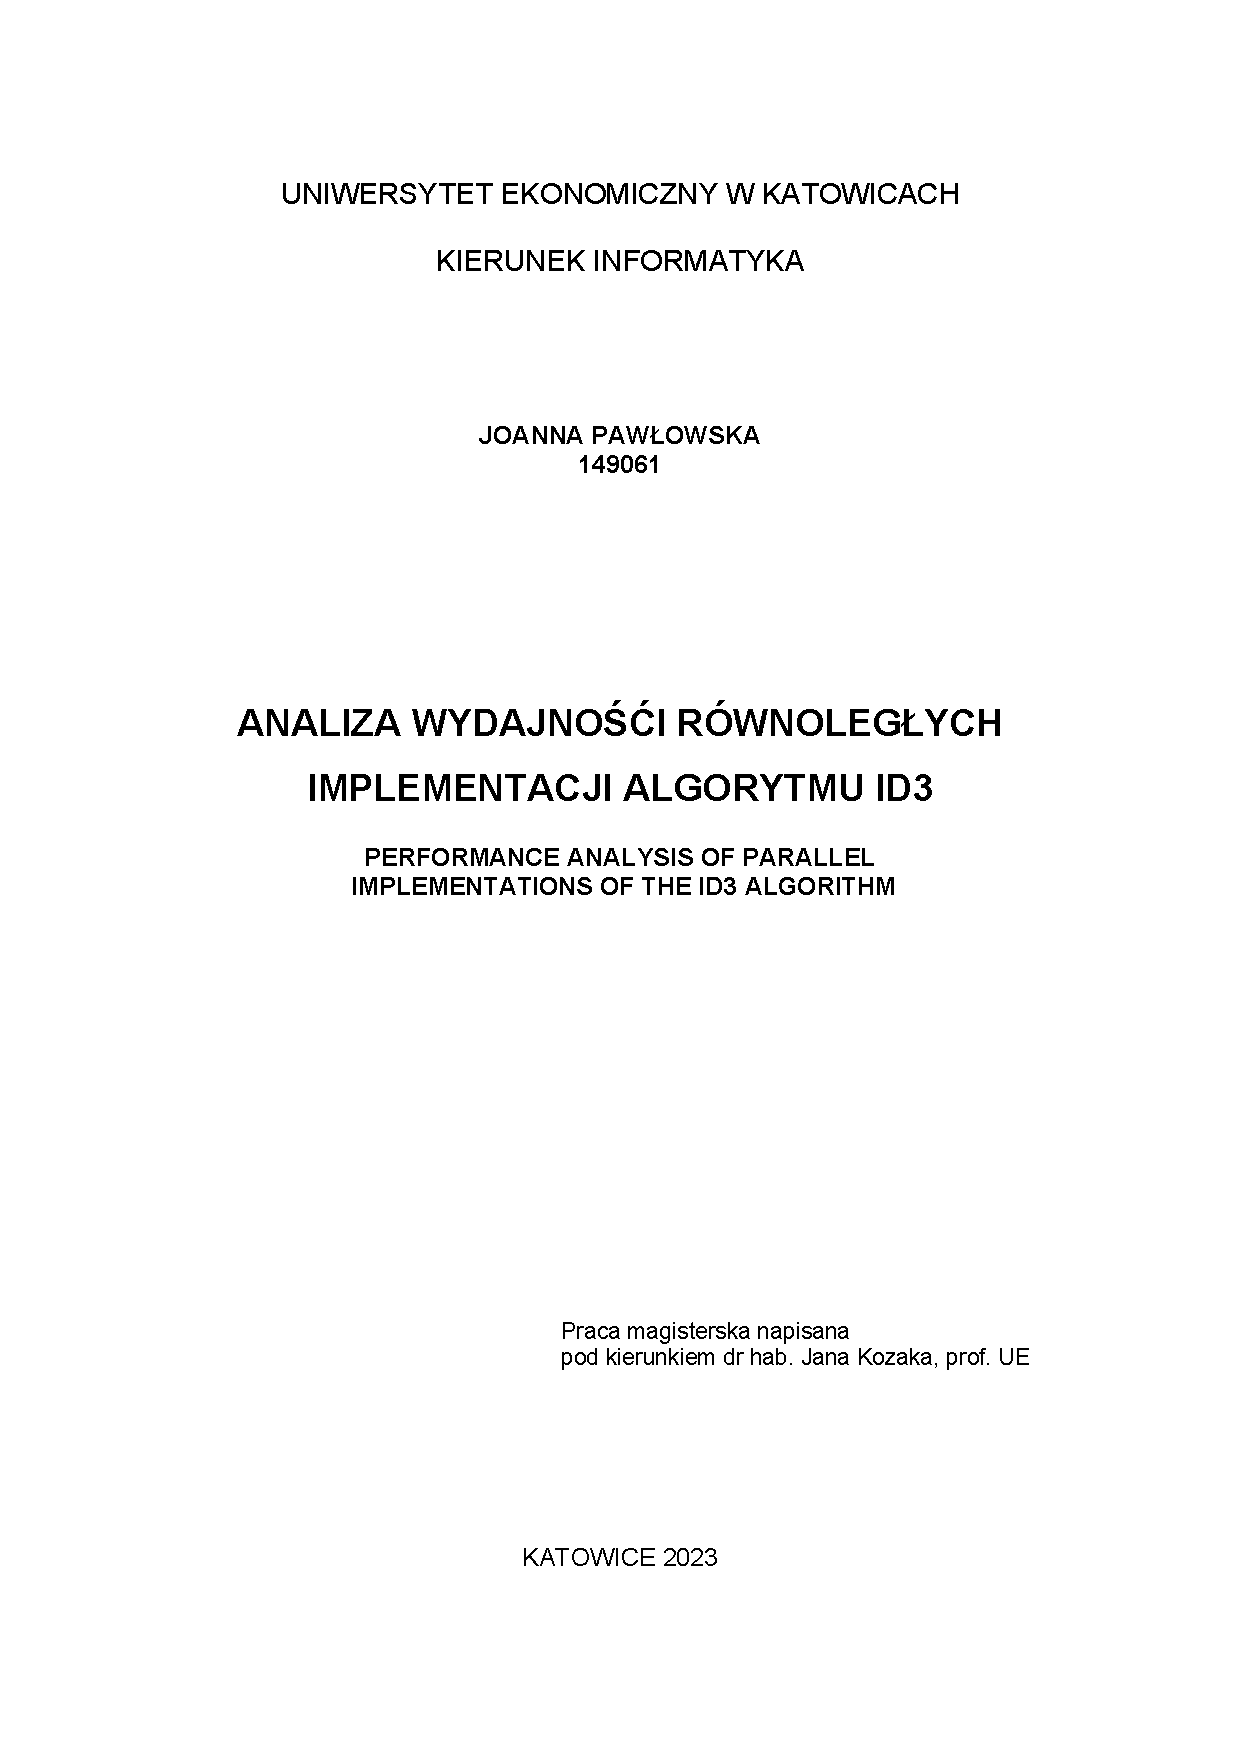
\includegraphics[width=\paperwidth,height=0.99\paperheight,keepaspectratio]{tytulowa.pdf}
\end{figure}
\newpage

\begin{figure}[H]
    \centering
	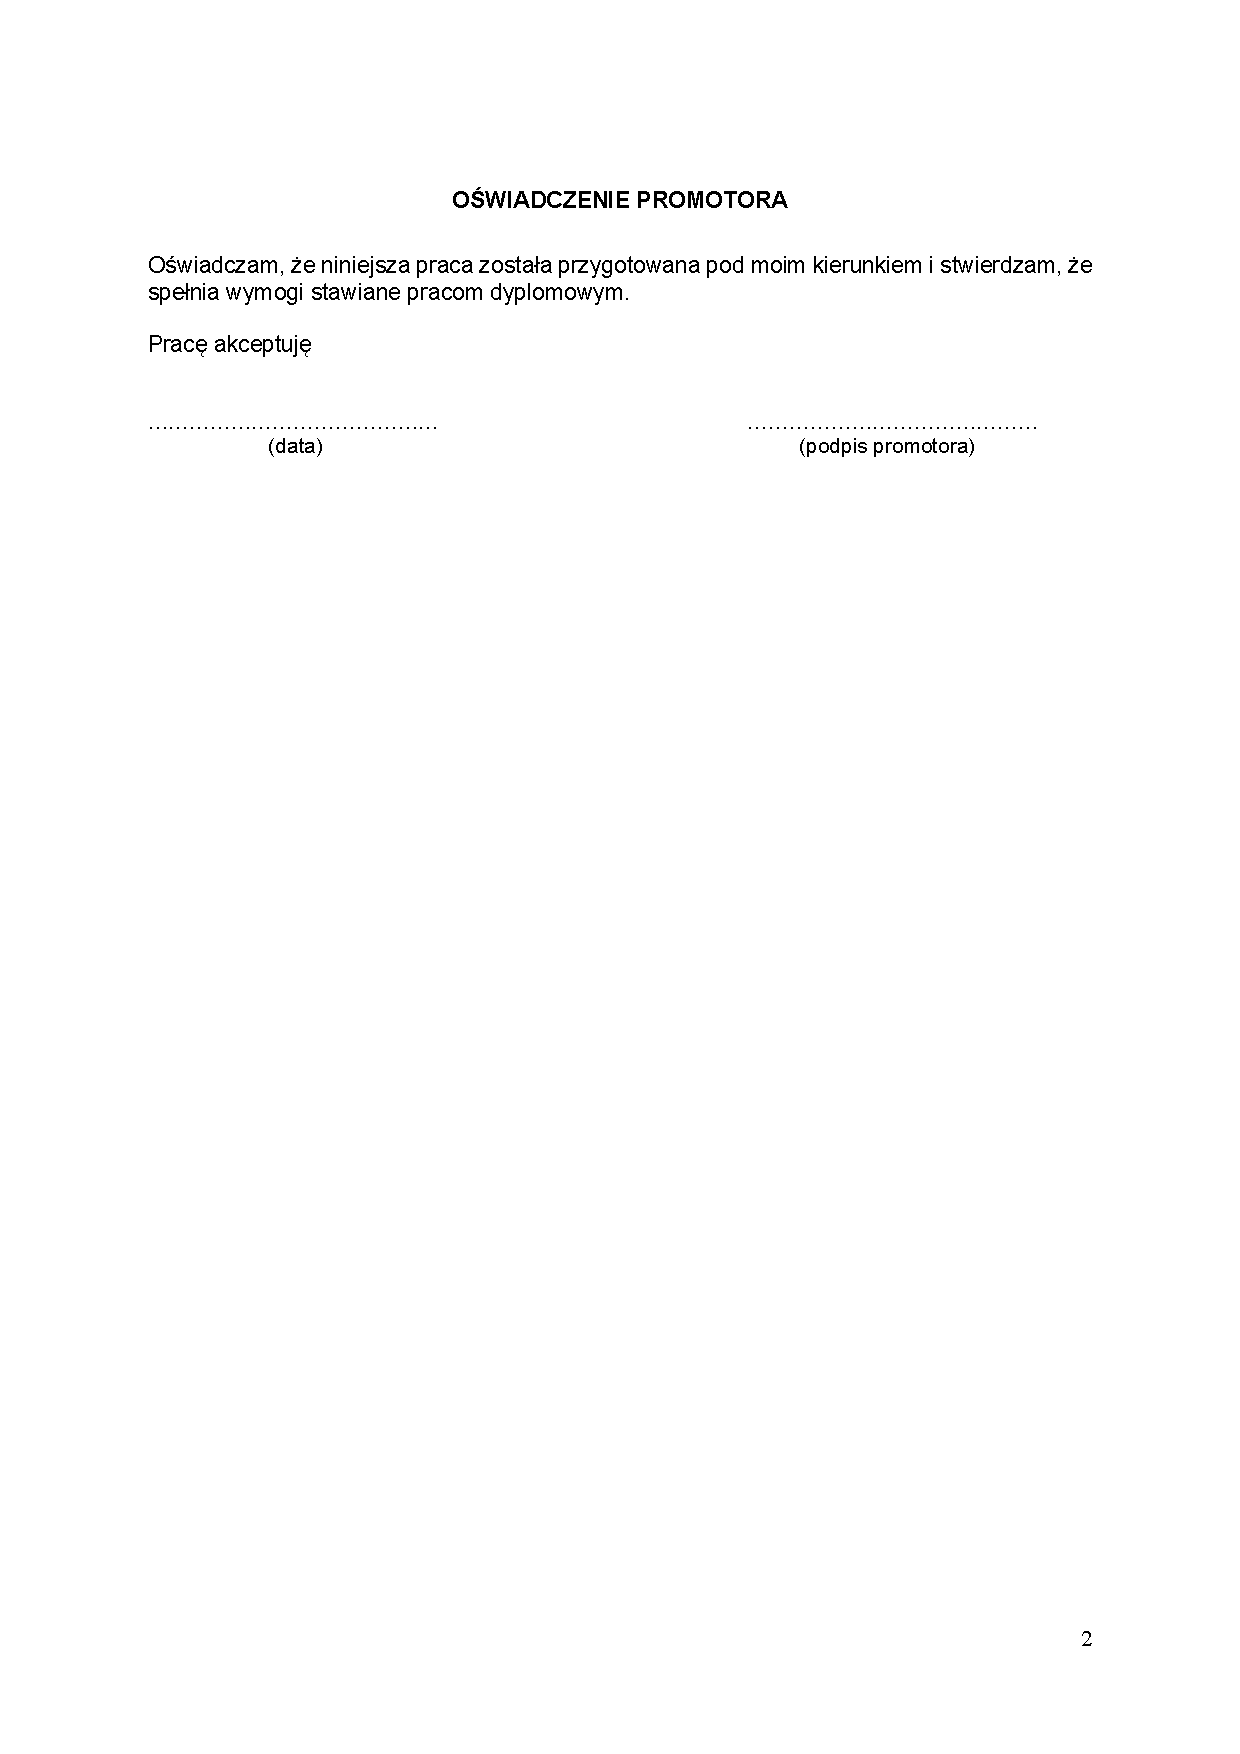
\includegraphics[width=\paperwidth,height=\paperheight,keepaspectratio]{oswiadczenie.pdf}
\end{figure}
\newpage

\begin{figure}[H]
    \centering
	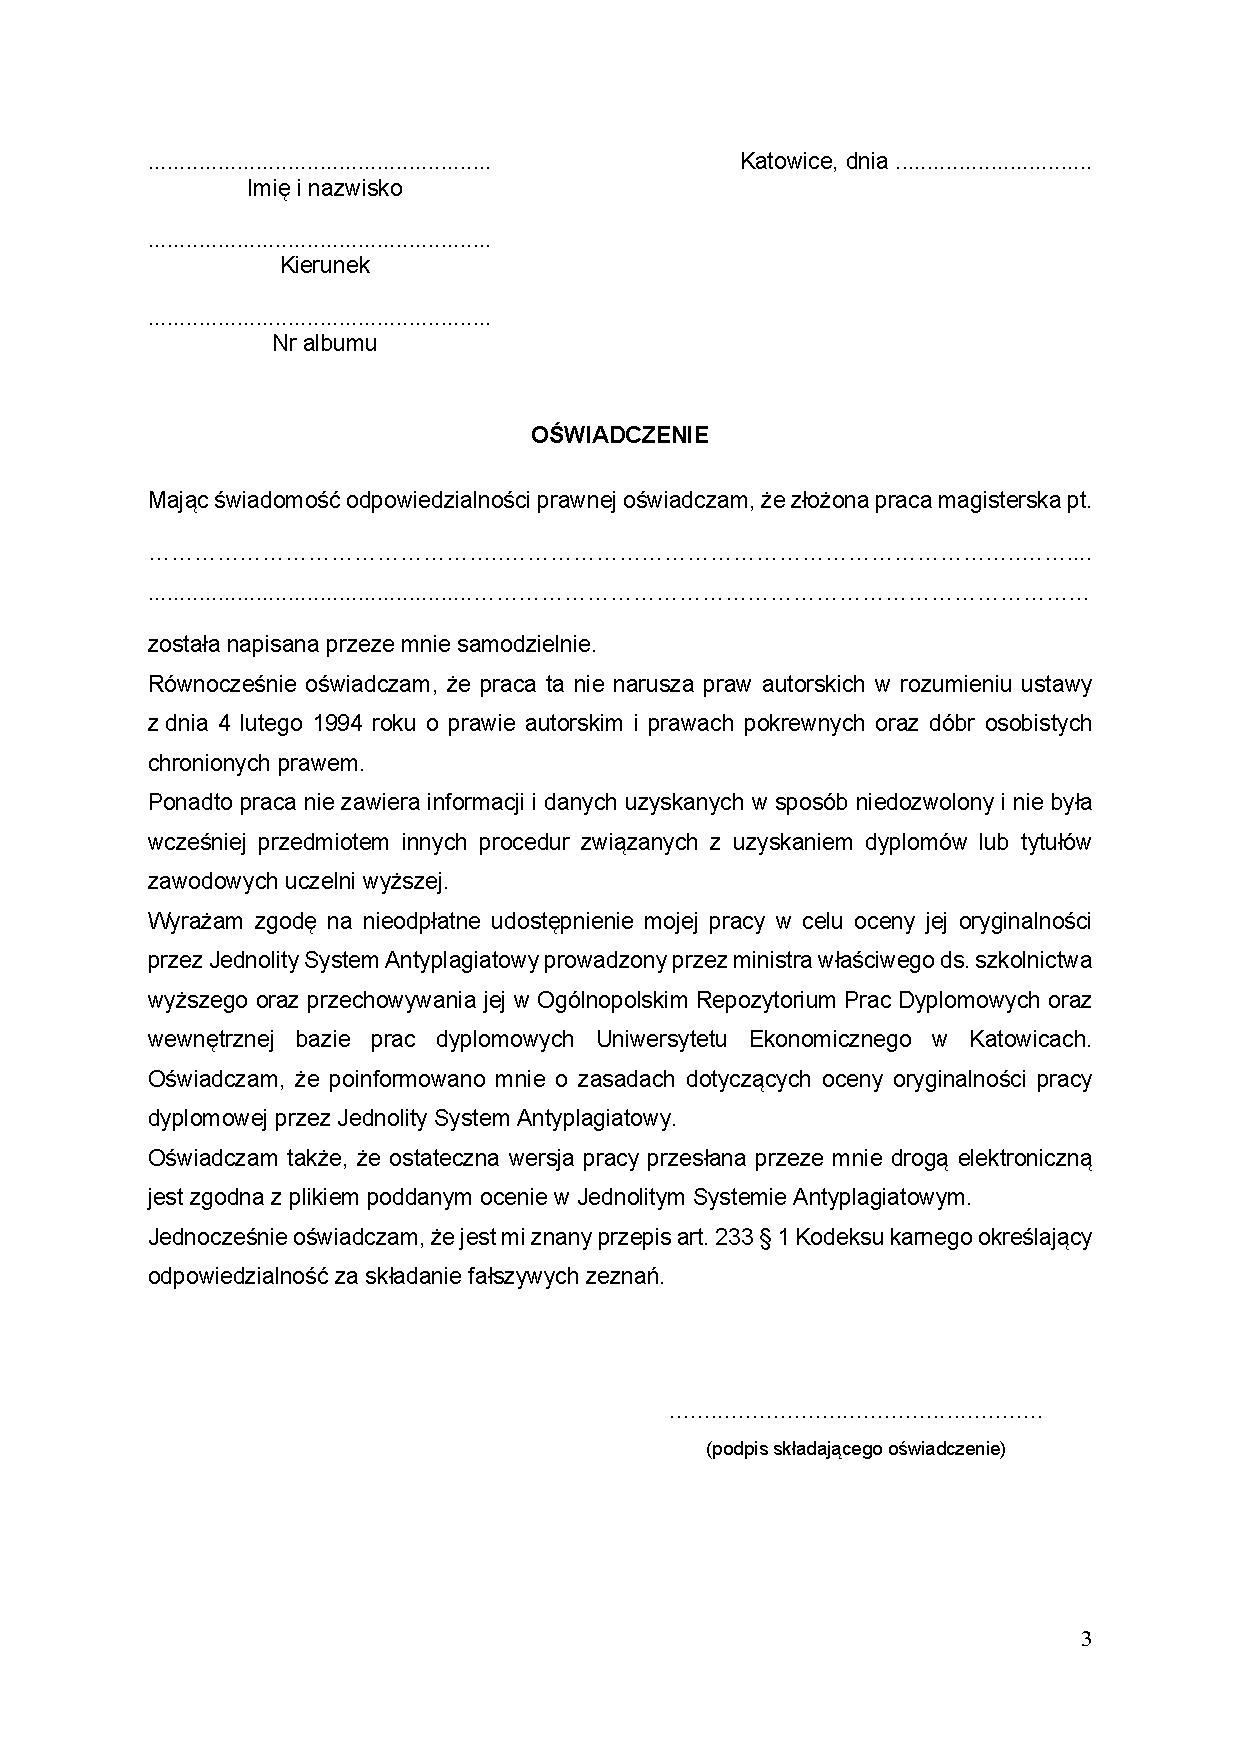
\includegraphics[width=\paperwidth,height=\paperheight,keepaspectratio]{plagiat.pdf}
\end{figure}
\newpage

\restoregeometry

% add table of contents
\tableofcontents
\newpage

\cleardoublepage
\phantomsection
\addcontentsline{toc}{section}{Wstęp}
\section*{Wstęp}
Równoległość jest techniką wykorzystywaną w wielu obszarach informatyki, dzięki której 
możliwe jest szybsze przetwarzanie danych oraz bardziej efektywne wykorzystanie zasobów komputera.
Stosowanie współbieżności w uczeniu maszynowym miało swoje początki już w~latach 80-tych XX wieku \cite{machine-learning-parallel-beginnings}.
Od tego czasu nastąpiło jednak wiele zmian zarówno technologicznych jak i w dziedzinie uczenia maszynowego.
Rozwój informatyki sprzętowej zapewnia większe możliwości w kontekście dostępnej mocy obliczeniowej.
Z kolei postęp w~obszarze uczenia maszynowego doprowadził do opracowania coraz bardziej skomplikowanych algorytmów, 
przetwarzających stale rosnące zbiory danych. Wszystkie te czynniki sprawiają, że~zagadnienie współbieżności w uczeniu 
maszynowym pozostaje ciągle istotne i aktualne.

Celem pracy jest zaproponowanie różnych implementacji algorytmu ID3 oraz analiza ich wydajności.
Punktem wyjściowym do porównania będzie implementacja sekwencyjna, w odniesieniu do której, porównane zostaną dwie implementacje równoległe.
Oczekiwanym rezultatem pracy jest przygotowanie dwóch równoległych wersji algorytmu, które w założeniu powinny okazać się bardziej
efektywne od wersji sekwencyjnej.

Praca składa się ze wstępu, pięciu rozdziałów oraz podsumowania. Pierwsze trzy
rozdziały wchodzą w skład teoretycznej części pracy. Rozdział czwarty oraz piąty
stanowią praktyczną część pracy.

Pierwszy rozdział poświęcony jest matematycznemu opisowi drzew decyzyjnych.
Przedstawiony został w nim schemat konstrukcji drzew decyzyjnych oraz różne algorytmy służące
do ich budowy. Rozdział drugi skupiony jest na zagadnieniach związanych z przetwarzaniem równoległym.
Zawiera on opis rodzajów procesów, sposoby dekompozycji problemów obliczeniowych a także
opis wzorców programowania równoległego. Rozdział trzeci prezentuje przegląd literatury 
na temat równoległych konstrukcji drzew decyzyjnych. W rozdziale czwartym przedstawione
zostały zaimplementowane wersje algorytmu ID3, które umożliwiają budowanie drzew decyzyjnych w sposób
sekwencyjny oraz równoległy. W ostatnim rozdziale omówiona została analiza wydajności zaimplementowanych
wersji algorytmu. Wyniki przeprowadzonych testów zaprezentowane zostały w formie graficznej.
Dodatkowo opisane zostały zaistniałe problemy implementacyjne. 
\newpage

\section{Drzewa decyzyjne}
Drzewo decyzyjne (ang. decision tree) to rodzaj algorytmu uczenia maszynowego
wykorzystywanego do klasyfikacji danych. Na podstawie danych wejściowych budowany jest model,
który pozwala na podejmowanie decyzji. Drzewo decyzyjne przedstawiane jest graficznie jako
struktura zbudowana z węzłów, gałęzi i liści. Każdy węzeł reprezentuje test, na podstawie
którego algorytm podejmuje decyzję. Gałęzie symbolizują możliwe wyniki testu. Ostateczne
decyzje, które mogą zostać podjęte przez algorytm, reprezentowane są przez liście.

Według matematycznej definicji drzewo decyzyjne to acykliczny graf skierowany.
Gałęzie odpowiadają krawędziom grafu. Wierzchołki grafu nazywane są węzłami. Węzły, które
nie mają żadnych potomków, określane są liśćmi, natomiast węzeł nieposiadający rodzica
nazywany jest korzeniem \cite{algorytmy-do-konstruowania-drzew-decyzyjnych}.

\subsection{Definicje}
Rekord (inaczej nazywany krotką, wierszem lub obiektem) jest wektorem wartości atrybutów.
Zbiór $n \in \mathbb{N}$ atrybutów wejściowych oznaczany jest przez $A = \{a_1, ..., a_i, ..., a_n\}$.
Atrybut $a_i$ przyjmuje wartości, których zbiór oznaczany jest przez
$dom(a_i) = \{v_{i,1}, v_{i,2}, ..., v_{i,|dom(a_i)|}\}$,
gdzie $|dom(a_i)|$ oznacza moc zbioru wartości atrybutu $a_i$. Atrybut wyjściowy nazywany
jest decyzją i oznaczany jest przez $y$. Możliwe wartości decyzji $dom(y) = \{c_1, ..., c_{|dom(y)|}\}$
nazywane są klasami decyzyjnymi. Przestrzeń rekordów wyznaczona jest jako iloczyn kartezjański
wszystkich zbiorów atrybutów wejściowych $X = dom(a_1) \times ... \times dom(a_i) \times ... \times dom(a_n)$
oraz zbioru atrybutów wyjściowych $dom(y)$ i oznaczana jest literą $U = X \times dom(y)$ \cite{data-mining-with-decision-trees}.

Zbiór danych $S$ to zbiór $m$ par takich, że $S = (\langle x_1, y_1\rangle, ..., \langle x_m, y_m\rangle)$,
gdzie: $m \in \mathbb{N} $, $x_q \in X$, $y_q \in dom(y)$. Zbiór $S$ graficznie przedstawiany jest jako tabela
i nazywany jest tabelą decyzyjną. Rekordy tworzą wiersze tabeli a kolumny grupują wartości atrybutów \cite{data-mining-with-decision-trees}.

\begin{table}[H]
    \centering
    $\begin{array}{|c|c|c|c|}
        \hline 
        a_1 & a_2 & a_3 & y \\
        \hline \hline
        v_{1,1} & v_{2,1} & v_{3,1} & c_1 \\
        v_{1,2} & v_{2,1} & v_{3,2} & c_3 \\
        v_{1,1} & v_{2,1} & v_{3,1} & c_1 \\
        v_{1,2} & v_{2,1} & v_{3,3} & c_3 \\
        v_{1,2} & v_{2,2} & v_{3,4} & c_2 \\
        \hline
    \end{array}$
    \caption{\label{tab:decision-table}Tabela decyzyjna dla $m=5$, $|dom(y)|=3$,\\ $|dom(a_1)|=2$, $|dom(a_2)|=2$, $|dom(a_3)|=4$ i $n=3$.}
\end{table}

Zazwyczaj zakłada się, że rekordy, które należą do
zbioru $S$ generowane są losowo zgodnie z pewnym nieznanym, wspólnym rozkładem prawdopodobieństwa $D$ nad przestrzenią $U$.
Selekcja $(\sigma)$ względem atrybutów przedstawiona jest za pomocą notacji używanej w algebrze.
Przykładowo wybranie z tabeli \ref{tab:decision-table} rekordów, które dla atrybutu $a_3$ przyjmują
wartość~$v_{3,1}$ opisywane jest wyrażaniem $\sigma_{a_3=v_{3,1}}S$.

Testem $t$ nazywany jest warunek dla podziału danych. W celu wyznaczenia najlepszego testu wykorzystywane
są różne kryteria podziału. Przy użyciu testów na atrybutach konstruowane jest drzewo decyzyjne $DT$.
Klasyfikator, który został stworzony ze zbioru danych $S$ oznaczany jest jako $DT(S)$. Korzystając z klasyfikatora
$DT(S)$ możliwe jest wyznaczenie predykcji $DT(S)(x_q)$ dla wybranego elementu $x_q \in X$. Rozmiar drzewa decyzyjnego $DT(S)$ oraz dokładność predykcji $DT(S)(x_q)$
w dużym stopniu zależy od wielkości zbioru $S$. Jeśli zbiór danych jest zbyt mały, to dokładność predykcji będzie niska.

Błąd klasyfikacji drzewa $DT(S)$ jest prawdopodobieństwem błędnej predykcji obiektu wybranego zgodnie z rozkładem $D$.
Błąd $\varepsilon$ zdefiniowany jest następująco (w przypadku atrybutów ciągłych znak sumy zastępowany jest całką):

\begin{equation}
    \varepsilon(DT(S), D) = \displaystyle\sum_{\langle x, y\rangle \in U} D(x, y) \cdot L(y, DT(S)(x)),
\end{equation}
\begin{equation}
    L(y, DT(S)(x)) = \left\{
        \begin{array}{ll}
            1, & DT(S)(x) = y, \\
            0, & DT(S)(x) \neq y.
        \end{array} \right.
\end{equation}

\vspace{0.8cm}

Dokładność klasyfikacji obliczana jest jako $1 - \varepsilon$.
Rzeczywista wartość błędu $\varepsilon$ jest jednak rzadko wyznaczana, ponieważ najczęściej rozkład $D$ nie jest znany.
W zamian, jako oszacowanie błędu klasyfikacji, korzysta się z błędu $\hat{\varepsilon}$
obliczanego tylko na zbiorze danych. Dokładność klasyfikacji wyznaczana jest wtedy jako $\frac{\hat{\varepsilon}}{|S|}$.

\begin{equation}
    \hat{\varepsilon}(DT(S), S) = \displaystyle\sum_{\langle x, y\rangle \in S} L(y, DT(S)(x)),
\end{equation}

\vspace{0.8cm}

Wykorzystywanie błędu $\hat{\varepsilon}$ wyliczanego na podstawie całego zbioru danych $S$ zazwyczaj daje jednak
zbyt optymistycznie oszacowanie błędu $\varepsilon$. Z tego powodu zbiór danych dzieli się na zbiór
treningowy oraz testowy. Zbiór treningowy jest większy i na jego podstawie buduje się klasyfikator.
Zbiór testowy wykorzystywany jest do wyliczania $\hat{\varepsilon}$, który zwykle zapewnia
lepsze oszacowanie błędu $\varepsilon$ \cite{data-mining-with-decision-trees}.

Nadmierne dopasowanie (ang. overfitting) to sytuacja, w której utworzony klasyfikator jest zbyt
dobrze dopasowany do danych treningowych. Wystąpienie nadmiernego dopasowania sprawia, że
klasyfikator dobrze sprawdza się dla danych treningowych, jednak zmniejsza się jego zdolność
generalizacji. Oznacza to, że dla elementu $x_q \in X$, mniejsze jest prawdopodobieństwo na otrzymanie
poprawnej predykcji $DT(S)(x_q)$. W przypadku drzew decyzyjnych nadmierne dopasowanie
występuje najczęściej, gdy drzewo ma zbyt wiele węzłów w stosunku do ilości dostępnych danych treningowych.

W celu uniknięcia lub minimalizacji zjawiska nadmiernego dopasowania stosuje się technikę przycinania drzewa (ang. pruning).
Polega ona na odpowiednim upraszczaniu drzewa poprzez zmniejszanie jego rozmiaru.
W drzewie decyzyjnym wycina się wybrane fragmenty (poddrzewa), których znaczenie jest niewielkie podczas przeprowadzania
predykcji obiektów. Poddrzewo, które zostało wybrane do wycięcia, najczęściej zastępuje się liściem z etykietą klasy, która
najczęściej występuje w wycinanym podzbiorze. Przekształcenia drzewa mogą pogorszyć dokładność klasyfikacji
na zbiorze danych treningowych, jednak często skutkują dokładniejszymi predykcjami na obiektach spoza zbioru treningowego.

\subsection{Schemat konstrukcji}
Proces budowania drzewa oparty jest na wielokrotnym podziale danych. Pierwszy krok polega na przypisaniu
korzeniowi wszystkich obiektów ze zbioru treningowego $S$. Następnie, stosując kryterium podziału zależne od
użytego algorytmu, wyznaczany jest atrybut wejściowy względem którego zostanie wykonany podział obiektów.
Najlepszym podziałem jest ten, który najmniej różnicuje obiekty ze względu na ich klasę decyzyjną.
Gdy wybrany zostanie atrybut, wykonywany jest test, który przydziela obiekty nowym węzłom potomnym.
Po dopasowaniu obiektów do nowych węzłów, proces podziału jest powtarzany według takiej samej zasady.
Podział wykonywany jest tak długo, aż osiągnięte zostanie kryterium stopu.

\subsubsection{Testy atrybutów}
Reguły definiujące podział w drzewach decyzyjnych są najczęściej jednowymiarowe.
Oznacza to, że test dokonywany jest na podstawie tylko jednego atrybutu.
Podziały wielowymiarowe są spotykane zdecydowanie rzadziej ze względu na wysoką złożoność obliczeniową \cite{eksploracja-danych}.
Testy dzieli się w zależności od rodzaju atrybutów. Wyróżniane są dwa różne podziały dla atrybutów typu dyskretnego i
dwa kolejne dla atrybutów ciągłych:
\newpage

\begin{itemize}

    \item dla atrybutów dyskretnych:
    \begin{itemize}
        \item podział oparty na wartościach atrybutu:
            $$t(x) = a_i(x),$$
            gdzie:\\
            $x \in X$,

        \item podział oparty na równości:
            $$  t(x) = \left\{
                \begin{array}{ll}
                1, & \textnormal{gdy } a_i(x) = v_{i,j}, \\
                0, & \textnormal{w przeciwnym wypadku,}
                \end{array} \right.
            $$
            gdzie:\\
            $v_{ij} \in dom(a_i)$,
    \end{itemize}

    \item dla atrybutów ciągłych:
    \begin{itemize}
        \item podział oparty na nierównościach:
            $$  t(x) = \left\{
                \begin{array}{ll}
                1, & \textnormal{gdy } a_i(x) \leqslant p, \\
                0, & \textnormal{w przeciwnym wypadku,}
                \end{array} \right.
            $$
            gdzie:\\
            $p \in dom(a_i)$ -- wartość progowa,

        \item podział oparty na przedziałach:
            $$  t(x) = \left\{
                \begin{array}{ll}
                1, & \textnormal{gdy } a_i(x) \in I_1, \\
                2, & \textnormal{gdy } a_i(x) \in I_2, \\
                3, & \textnormal{gdy } a_i(x) \in I_3, \\
                \vdots & \\
                k, & \textnormal{gdy } a_i(x) \in I_l, \\
                
                \end{array} \right.
            $$
            gdzie:\\
            $l \in \mathbb{N}$,\\
            $I_1, I_2, I_3, ..., I_l \subset dom(a_i)$, \\
            $j \neq k \implies I_j \cap I_k = \varnothing$.
    \end{itemize}

\end{itemize}

\subsubsection{Kryteria stopu}
Faza rozbudowy drzewa trwa do momentu, gdy któryś z warunków stopu zostanie spełniony.
Wyróżnia się następujące kryteria zatrzymania konstruowania drzewa decyzyjnego:
\begin{itemize}
    \item pusty zbiór treningowy,
    \item jednorodność obiektów - wszystkie rekordy mają taką samą wartość $y$ (należą do tej samej klasy decyzyjnej),
    \item drzewo osiągnęło maksymalną wysokość,
    \item brak możliwość odnalezienia testu, który pozwoliłby na dokonanie podziału \cite{data-mining-with-decision-trees}.
\end{itemize}

\subsubsection{Ocena jakości}
Dwie składowe, które wpływają na ocenę jakości $Q$ drzewa decyzyjnego $DT(S)$, to dokładność klasyfikacji oraz wielkość drzewa decyzyjnego.
Wielkość drzewa decyzyjnego wyznaczana jest na różne sposoby. Miarą może być wysokość drzewa, liczba węzłów
lub liczba liści. We wszystkich przypadkach występuje jednak taka sama zasada -- im mniejsze drzewo, które
umożliwia przeprowadzanie poprawnych predykcji, tym wyższa jest jego jakość. Jakość drzewa decyzyjnego może oceniona być za pomocą (\ref{Q}):


\begin{equation}\label{Q}
Q(DT, S) = \alpha \cdot  \hat{\varepsilon}(DT(S), S) + \beta \cdot h(DT),
\end{equation}
gdzie: \\
$\alpha$, $\beta$ $\in \mathbb{R}$,\\
$h$ -- wysokość drzewa decyzyjnego.

\subsection{Algorytmy konstrukcji drzew decyzyjnych}

\textbf{Algorytm ID3} jest uważany za jeden z prostszych algorytmów konstrukcji drzew decyzyjnych.
Jako kryterium podziału wykorzystany jest zysk informacji $InformationGain$, który obliczany jest
przy wykorzystaniu entropii $H$:

\begin{equation}
    H(y, S) = - \displaystyle\sum\limits_{c_j \in dom(y)}^{} \frac{\sigma_{y=c_j}S}{|S|} \cdot log_2 \frac{\sigma_{y=c_j}S}{|S|},
\end{equation}

\begin{equation}
    InformationGain(a_i, S) = H(y, S) - \displaystyle\sum\limits_{v_{i,j} \in dom(a_i)}^{} \displaystyle\frac{\sigma_{a_i=v_{i,j}}S}{|S|} \cdot H(y, \sigma_{a_i=v_{i,j}}S).
\end{equation}

Atrybut $a_i$ dla którego zysk informacji jest najwyższy wybierany jest do wyznaczenia podziału.
Budowanie drzewa kończy się, gdy wszystkie obiekty w węźle mają taką samą wartość
klasy lub gdy najlepszy obliczony zysk informacji nie jest większy od zera \cite{algorytmy-do-konstruowania-drzew-decyzyjnych}.

Algorytm stosowany jest dla atrybutów dyskretnych. Jeśli atrybuty są ciągłe, wówczas muszą
zostać przekształcone. ID3 nie sprawdza się w przypadku, gdy zbiór treningowy składa się z
rekordów, którym brakuje wartości pojedynczych atrybutów. ID3 jest algorytmem zachłannym,
dlatego nie daje gwarancji odnalezienia rozwiązania optymalnego, ponieważ może
utknąć w optimum lokalnym \cite{data-mining-with-decision-trees}.

\textbf{Algorytm C4.5} jest ulepszoną wersją ID3 zaproponowaną przez tego samego autora.
Jako kryterium podziału wykorzystany został współczynnik względnego zysku informacji $GainRatio$, który zdefiniowany jest następująco:

\begin{equation}
    GainRatio(a_i, S) = \displaystyle\frac{InformationGain(a_i, S)}{H(a_i, S)},
\end{equation}

\vspace{0.8cm}

W przeciwieństwie do algorytmu ID3, algorytm C4.5 może przetwarzać zarówno atrybuty dyskretne jak i ciągłe.
Obsługa atrybutów ciągłych uzyskiwana jest poprzez podział wartości atrybutu
na dwa podzbiory zgodnie z najlepszym znalezionym progiem.
Dodatkowo jest on dostosowany do obsługi rekordów z brakującymi wartościami atrybutów. Kolejnym usprawnieniem
jest zastosowanie procedury przycinania. Pozwala ona na usuwanie gałęzi wraz z~połączonymi węzłami potomnymi, które
nie przyczyniają się do poprawienia dokładności klasyfikatora i zastępowanie ich jednym węzłem liścia.
Komercyjnie wykorzystuje się \textbf{algorytm C5.0}, który jest zaktualizowaną wersją algorytmu C4.5.
Jest on zoptymalizowany pod kątem czasu obliczeń i wykorzystanej pamięci \cite{data-mining-with-decision-trees}.

\textbf{Algorytm CART} pozwala na konstruowanie drzew opartych są na binarnym podziale 
atrybutów. Kryterium podziału wykorzystuje indeks $Gini$, który mierzy
rozbieżności między rozkładami prawdopodobieństwa wartości atrybutów.
Kryterium oceny wyboru atrybutu $a_i$ zdefiniowane jest jako $ GiniGain$ \cite{data-mining-with-decision-trees}:

\begin{equation}
    Gini(y, S) = 1 - \displaystyle\sum\limits_{c_j \in dom(y)}^{} \Bigg(\displaystyle\frac{|\sigma_{y=c_j}S|}{|S|}\Bigg)^2,
\end{equation}

\begin{equation}
    GiniGain(a_i, S) = Gini(y, S) - \displaystyle\sum\limits_{v_{i,j} \in dom(a_i)}^{} \displaystyle\frac{|\sigma_{a_i=v_{i,j}}S|}{|S|} \cdot Gini(y, \sigma_{a_i=v_{i,j}}S)
\end{equation}

\vspace{0.8cm}

Podobnie jak w algorytmie C4.5 dopuszczalne są zarówno atrybuty dyskretne jak i ciągłe.

\newpage

\textbf{Algorytm CHAID} (ang. Chi-squared Automatic Interaction Detectorest) to jeden z~najstarszych algorytmów budowy drzew decyzyjnych, który można wykorzystać 
zarówno dla atrybutów ciągłych jak i dyskretnych. Drzewa stworzone przy wykorzystaniu algorytmu~CHAID są drzewami niebinarnymi.

Dla każdego atrybutu $a_i$ znajdywana jest para wartości $\langle v_{ij}, v_{ik}\rangle$, która jest najmniej różna w odniesieniu do decyzji.
Różnica jest mierzona poprzez wykonanie testu statystycznego, którego wybór zależy od rodzaju atrybutu wyjściowego.
Gdy jest on typu dyskretnego kryterium podziału opiera się na teście $Chi$-kwadrat, w przeciwnym wypadku wykorzystuje się test $F$.

Dla każdej pary wartości sprawdza się, czy wynik testu statystycznego jest większy od~progu scalania.
Jeśli wynik testu jest większy to wartości są łączone, a następnie ponownie wykonuje się proces wyboru pary.
Proces powtarza się do momentu, gdy nie będzie możliwe odnalezienie żadnej znaczącej pary.
Następnie wybierany jest najlepszy atrybut wejściowy, który zostanie użyty do podziału bieżącego węzła,
tak aby każdy węzeł potomny składał się z grupy jednorodnych
wartości wybranego atrybutu \cite{data-mining-with-decision-trees}.

Algorytm CHAID obsługuje brakujące wartości, które traktuje jako jedną kategorie. W~algorytmie nie stosuje się przycinania.

\newpage
\section{Programowanie równoległe}
Rozdział ma na celu uporządkowanie istotnych pojęć związanych z tematem programowania
równoległego. Opisane zostały podstawowe zagadnienia, różnice między programowaniem współbieżnym
i równoległym, rodzaje dekompozycji zadań, a także wzorce, stosowane w równoległych 
implementacjach algorytmów.

\subsection{Podstawowe pojęcia}
Przetwarzanie równoległe jest tematem omawianym w ramach dziedziny systemów operacyjnych.
Mimo, że celem pracy nie jest analiza zagadnień specyficznych dla systemów operacyjnych,
poniżej przestawione zostały pojęcia, których zrozumienie jest konieczne do~tworzenia 
równoległych implementacji algorytmów.

\textbf{Procesor} to jednostka sprzętowa, która pobiera dane z pamięci operacyjnej, interpretuje je
i wykonuje. Pojęcie procesor używane jest w dwóch kontekstach. Pierwszy, zgodny z podaną definicją, używany
jest głównie w elektronice. Drugie znaczenie procesora wykorzystywane jest częściej w programowaniu.
Wówczas pojęcie procesor jest synonimem pojęcia rdzeń.

\textbf{Rdzeniem fizycznym} (ang. core) określany jest fizyczny element procesora, który pozwala na wykonywanie obliczeń.
W uproszczeniu, im więcej rdzeni posiada procesor, tym więcej obliczeń może on wykonać w jednostce czasu, co definiowane
jest jako moc obliczeniowa. Jest to jeden z czynników branych pod uwagę przy ocenie wydajności procesora. Obecnie używa się
głównie procesorów wielordzeniowych.

\textbf{Rdzeń logiczny} (ang. logical core, thread) przygotowuje dane wykorzystywane podczas obliczeń wykonywanych przez rdzeń fizyczny.
Do niedawna na jeden rdzeń fizyczny przypadał jeden rdzeń logiczny.
Obecnie najczęściej każdemu rdzeniowi fizycznemu przypisuje się dwa rdzenie logiczne.
Rdzenie logiczne uzależnione są od rdzenia fizycznego, do którego są przypisane, natomiast nie są zależne
od operacji rdzeni logicznych przypisanych do innego rdzenia fizycznego.

\textbf{Rozkazem} nazywane jest pojedyncze polecenie, zapisane jest w postaci liczb binarnych, które
wykonywane jest przez procesor.

\textbf{Instrukcja} definiowana jest jako bardziej złożone zadanie, które składa się ze zbioru rozkazów. Instrukcje
mogą być niskopoziomowe (napisane w np. języku \textit{Asembler}) lub wysokopoziomowe (napisane w językach np. \textit{C} i \textit{Java}).
Instrukcje wysokopoziomowe tłumaczone są na kilka instrukcji niskopoziomowych, natomiast instrukcje
niskopoziomowe tłumaczone są na zbiór rozkazów. Zbiór rozkazów może być dzielony na podzbiory w celu
uruchomienia każdego podzbioru na innym procesorze.

\textbf{Program} jest zbiorem instrukcji, który pozwala na rozwiązanie pewnego problemu obliczeniowego. 

\textbf{Proces} najprościej definiowany jest jako program, który jest w trakcie wykonywania. Pod pojęciem procesu zawiera
się jednak wiele mechanizmów, przy pomocy których system operacyjny zarządza wykonywaniem programu.
System operacyjny przydziela każdemu nowemu procesowi zasoby m.in. odrębny obszar pamięci operacyjnej, nadaje
unikatowy numer PID~(ang. process identifier), kontroluje stan procesu oraz zarządza plikami, z których korzysta proces \cite{programowanie-rozproszone-i-rownolegle}.

\textbf{Wątek} (ang. thread) jest częścią procesu. Jest to niezależny strumień instrukcji, który uruchamiany jest przez system operacyjny.
Na jeden proces najczęściej składa się wiele strumieni instrukcji. Instrukcje składające się na wątek są wykonywane sekwencyjnie.
Wszystkie wątki istniejące w ramach jednego procesu współdzielą przestrzeń adresową -- mają dostęp do pamięci wspólnej.
Z tego powodu komunikacja między wątkami należącymi do jednego procesu jest łatwa i nie wymaga wsparcia systemu operacyjnego.
Przekazanie danych polega na podaniu jedynie wskaźnika do miejsca w pamięci.
Programiści często definiują wątek nieco inaczej. Wątek traktowany jest jako nieblokująca metoda, która wykonywana jest
niezależnie od procesu, który ją uruchomił \cite{programowanie-rozproszone-i-rownolegle}. Określenie wątek jest również używane
wymiennie z określeniem rdzeń logiczny. Wątek w znaczeniu rdzenia logicznego nie jest jednak równoznaczny przedstawionej definicji wątku.

\subsection{Rodzaje procesów}

\textbf{Proces sekwencyjny} $P$ charakteryzuje się tym, że każda kolejna instrukcja $i$ wykonywana jest dopiero wtedy, gdy zakończy
się wykonywanie poprzedniej. Kolejność wykonywania instrukcji jest jednoznacznie określona, dlatego proces sekwencyjny
określany jest jako pojedynczy ciąg instrukcji \cite{wprowadzenie-do-obliczen-rownoleglych}. W przypadku procesu sekwencyjnego
wątek nie jest częścią procesu, natomiast jest z nim utożsamiany \cite{skrypt}. Schemat przykładowego procesu sekwencyjnego
przedstawiony jest na rysunku \ref{fig:sequential}.

\begin{figure}[H]
    \centering
	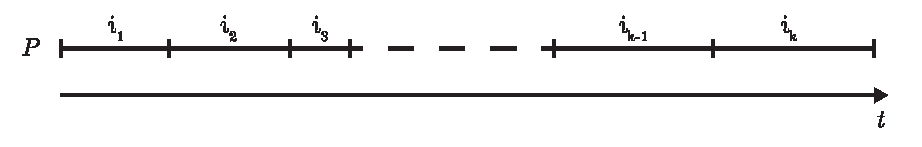
\includegraphics[width=\textwidth]{sequential.pdf}
    \caption{Proces sekwencyjny. Źródło: Opracowanie własne na podstawie \cite{wprowadzenie-do-obliczen-rownoleglych}}
    \label{fig:sequential}
\end{figure}

\newpage 

Procesy sekwencyjne, które zachodzą na siebie w czasie, określane są jako \textbf{proces współbieżny}. Innymi słowami
proces współbieżny to proces, który składa się z wielu strumieni instrukcji.
Instrukcje należące do jednego wątku, wykonywane są, zanim ukończone zostanie wykonywanie
wszystkich instrukcji tworzących drugi, wcześniej uruchomiony wątek.

Dane są dwa procesy sekwencyjne $P_1$ i $P_2$, instrukcje $i_{1,1}, i_{1,2} \in P_1$ oraz $i_{2,1}, i_{2,2} \in P_2$.
Rysunek \ref{fig:concurrent} przedstawia jedną z wielu możliwych realizacji procesu $P_1$ oraz $P_2$.

\begin{figure}[H]
    \centering
	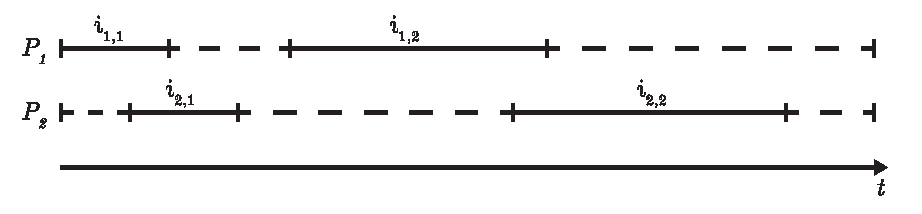
\includegraphics[width=\textwidth]{concurrent.pdf}
    \caption{Proces współbieżny. Źródło: Opracowanie własne na podstawie \cite{wprowadzenie-do-obliczen-rownoleglych}}
    \label{fig:concurrent}
\end{figure}

\textbf{Procesy wykonywane w przeplocie} są procesami współbieżnymi, w których wątki uruchamiane są naprzemiennie. Podczas wykonywania procesu $P_1$
następuje wstrzymanie procesu $P_2$. Gdy przerywane jest działanie procesu $P_1$ to przez pewien czas wykonywany
jest proces $P_2$. Metoda przeplotu pozwala na zastosowanie współbieżności w procesorach jednordzeniowych.
Rysunek \ref{fig:overlapping} prezentuje schemat procesów wykonywanych w przeplocie.

\begin{figure}[H]
    \centering
	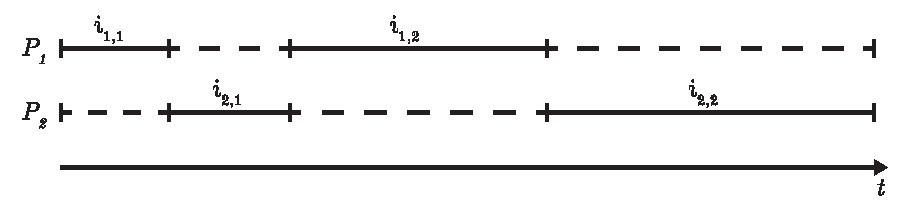
\includegraphics[width=\textwidth]{overlapping.pdf}
    \caption{Procesy wykonywane metodą przeplotu.\\ Źródło: Opracowanie własne na podstawie \cite{wprowadzenie-do-obliczen-rownoleglych}}
    \label{fig:overlapping}
\end{figure}

\textbf{Proces równoległy} jest szczególnym rodzajem procesu współbieżnego, w którym wątki uruchamiane są jednocześnie. Jeśli wątki mają zostać
rozdzielone między różne rdzenie procesora, wówczas konieczne jest wykorzystanie procesora z kilkoma rdzeniami. Inną możliwością jest zastosowanie architektury
rozproszonej. W takiej sytuacji wątki dzielone są między zbiór komputerów, które połączone są ze sobą siecią. Proces równoległy nazywany jest wtedy rozproszonym.
Na rysunku \ref{fig:parallel} przedstawione zostały procesy równoległe.

\begin{figure}[H]
    \centering
	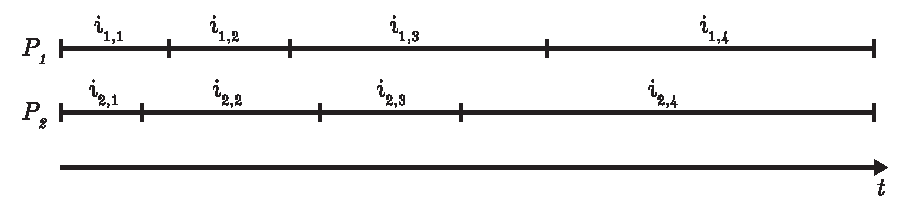
\includegraphics[width=\textwidth]{parallel.pdf}
    \caption{Procesy równoległe. Źródło: Opracowanie własne na podstawie \cite{wprowadzenie-do-obliczen-rownoleglych}}
    \label{fig:parallel}
\end{figure}

\subsection{Rodzaje dekompozycji problemów obliczeniowych}
W celu równoległego wykonywania programu istotne jest zaprojektowanie podziału zadań obliczeniowych. Podział problemu na
zadania nazywany jest dekompozycją. Wyróżniane są cztery rodzaje dekompozycji \cite{wprowadzenie-do-obliczen-rownoleglych}.

\textbf{Dekompozycja danych} to jeden z najczęściej wykorzystywanych rodzajów dekompozycji. Swoje zastosowanie znajduje szczególnie w przypadkach,
gdzie przetwarzane są bardzo duże ilości danych. Dekompozycja danych dzieli się na dekompozycję danych wejściowych i~wyjściowych.
Pierwsza z nich polega na podziale danych wejściowych na względnie równe części, które przetwarzane są w ramach osobnych zadań. Najczęściej
zadania polegają na~wykonaniu dokładnie takiego samego rodzaju obliczeń. Taki rodzaj dekompozycji charakteryzuje się tym,
że po zakończeniu zadań, konieczne jest ich zsumowanie.

Dekompozycja danych wyjściowych jest możliwa, gdy elementy danych wyjściowych mogą zostać wyznaczone niezależnie od siebie.
Wówczas każdemu zadaniu przydzielone zostają te~dane wejściowe, które konieczne są do otrzymania poszczególnych elementów
danych wyjściowych. Wadą takiego podejścia jest stosunkowo niski stopień współbieżności \cite{wprowadzenie-do-obliczen-rownoleglych}.

Podejście, w którym zrównoleglanie osiągane jest poprzez zastosowanie dekompozycji danych, określany jest pojęciem
\textit{równoległość danych}. 

\textbf{Dekompozycja funkcjonalna} polega na wyodrębnieniu obliczeń, których wykonanie konieczne jest do rozwiązania problemu. Obliczenia dzielone są
na grupy, które formowane są w funkcje. Zadania funkcji różnią się od siebie i najczęściej przetwarzają różne rodzaje danych
\cite{wprowadzenie-do-obliczen-rownoleglych}.
Zastosowanie dekompozycji funkcjonalnej oznacza wykorzystanie \textit{równoległości zadań}.

\textbf{Dekompozycja rekursywna} stosowana jest przy rozwiązywaniu problemów metodą ,,dziel i zwyciężaj". Problem dzielony jest na
mniejsze podproblemy, które są od siebie niezależne. Każdy podproblem jest mniejszym przypadkiem pierwotnego problemu. Podział
wykonywany jest tak długo, aż podproblemy stają się trywialne do rozwiązania. Następnie wszystkie rozwiązania scalane są w jedno,
które jest ostatecznym rozwiązaniem \cite{wprowadzenie-do-obliczen-rownoleglych}.

\textbf{Dekompozycja eksploracyjna} używana jest wtedy, gdy zadanie obliczeniowe polega na~przeszukiwaniu przestrzeni rozwiązań. Przestrzeń dzielona
jest na części, które eksplorowane są równolegle przez odrębne zadania. Jeśli rozwiązanie zostanie znalezione w którejś części przestrzeni,
wówczas wykonywanie pozostałych zadań jest przerywane \cite{wprowadzenie-do-obliczen-rownoleglych}.

\subsection{Wzorce programowania równoległego}
Istnieje wiele wzorców programowania równoległego. Podczas implementacji algorytmu równoległego ciężko jest dobrać jeden, najlepiej pasujący wzorzec.
Z tego powodu wzorce traktowane są raczej jako ogólne wskazówki, które mogą być przydatne podczas projektowania algorytmu. Najczęściej programy
tworzone są zgodnie z kilkoma wzorcami, które łączone są ze sobą w celu stworzenia implementacji dopasowanej do konkretnego przypadku.
W tym rozdziale opisane zostały wybrane wzorce programowania równoległego.

\subsubsection{Wzorzec Master-Slave}
Wzorzec \textit{Master-Slave}, zaprezentowany na rysunku \ref{fig:master-slave}, inaczej nazywany jest wzorcem \textit{Manager-Worker}. Wątek, który nazywany jest zarządcą (ang. master/manager)
definiuje zadania i rozdziela je pomiędzy wykonawców (ang. worker/slave). Gdy wykonawca zrealizuje zadanie, przesyła
otrzymane wyniki zarządcy, którego zadaniem jest scalić wszystkie zgromadzone wyniki w jedno rozwiązanie problemu.
Wzorzec nie sprawdza się w problemach o~dużym rozdrobnieniu zadań. Wówczas dochodzi do sytuacji, w której wykonawcy realizują poszczególne zadania
szybciej, niż zarządca jest w stanie je generować i rozdzielać \cite{wprowadzenie-do-obliczen-rownoleglych}.

\begin{figure}[H]
    \centering
	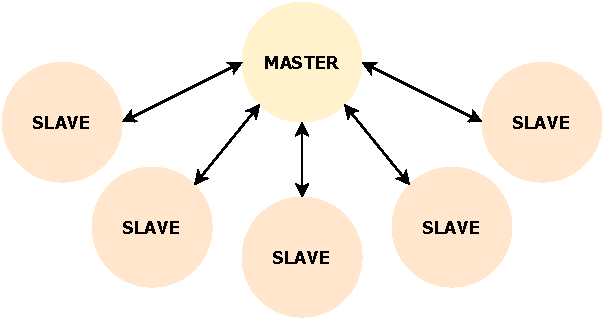
\includegraphics[width=0.5\textwidth]{patterns-master-slave.pdf}
    \caption{Wzorzec \textit{Master-Slave}. Źródło: Opracowanie własne.}
    \label{fig:master-slave}
\end{figure}

\subsubsection{Wzorzec Fork-Join}
Wzorzec \textit{Fork-Join} to jeden z najczęściej stosowanych wzorców. Wykonywanie programu rozpoczyna się
w ramach jeden wątku głównego. W momencie, gdy w kodzie programu pojawia się instrukcja, która wymaga
równoległego przetwarzania, tworzone są dodatkowe wątki poboczne. Sytuacja ta zaprezentowana jest na rysunku \ref{fig:fork-join}. Dopóki wszystkie
wątki poboczne nie zakończą równoległej pracy i nie zostaną zniszczone, wątek główny nie może wznowić wykonywania
sekwencyjnej części kodu. Etap ,,fork" polega na ustaleniu argumentów, które następnie otrzymuje każdy wątek.
Etap ,,join" łączy wyniki po zakończeniu pracy wszystkich wątków równoległych. Etapy ,,fork" i ,,join"
mogę wykonywane być dowolną liczbę razy \cite{parallel-design-patterns}.

\begin{figure}[H]
    \centering
	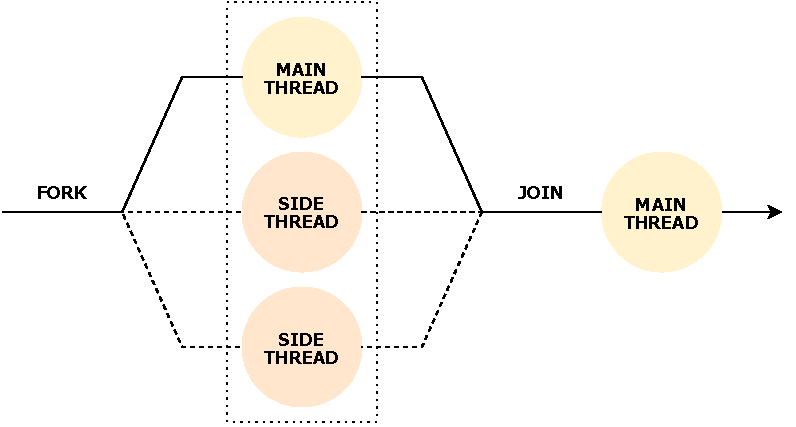
\includegraphics[width=0.6\textwidth]{patterns-fork-join.pdf}
    \caption{Wzorzec \textit{Fork-Join}. Źródło: Opracowanie własne.}
    \label{fig:fork-join}
\end{figure}

\subsubsection{Wzorzec Map-Reduce}
Wzorzec \textit{Map-Reduce} jest podobny do wzorca \textit{Fork-Join} \ref{fig:fork-join}. Dane wejściowe są przetwarzane równolegle przez wiele wątków.
Następnie wszystkie uzyskane wyniki są łączone, aż~do~momentu uzyskania jednego rozwiązania.
W działaniu obydwa wzorce są prawie identycznie, jednak wywodzą się z różnych pomysłów.
Idea mapowania pochodzi z technik stosowanych w~funkcjonalnych językach programowania.
Kilka mapowań może być połączonych w łańcuchy składające się na większe funkcje.
Etapy ,,map" i ,,reduce" są od siebie bardziej niezależne niż etapy ,,fork" i ,,join".
Mapowanie może występować bez redukcji, a redukcja bez mapowania~\cite{parallel-design-patterns}.
Graficzne przedstawienie wzorca \textit{Map-Reduce} zaprezentowane jest na rysunku \ref{fig:map-reduce}.

\begin{figure}[H]
    \centering
	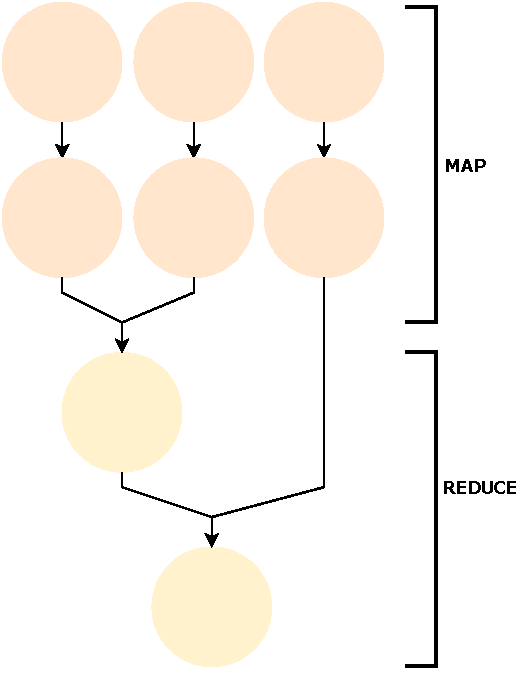
\includegraphics[width=0.4\textwidth]{patterns-map-reduce.pdf}
    \caption{Wzorzec \textit{Map-Reduce}. Źródło: Opracowanie własne.}
    \label{fig:map-reduce}
\end{figure}

\subsubsection{Wzorzec Work Pool}\label{work-pool}
Wzorzec puli zadań \textit{Work Pool} wykorzystywany jest w algorytmach, w których zadania generowane są dynamicznie
lub gdy istotnie różnią się złożonością. Zadania przechowywane są w strukturze danych, która dostępna
jest w pamięci współdzielonej. Najczęściej wykorzystywane struktury to lista, kolejka priorytetowe
czy tablica z haszowaniem. W momencie, gdy wątek zakończył obliczanie zadania, dostarczane jest mu
kolejne zadanie przechowywane w strukturze \cite{wprowadzenie-do-obliczen-rownoleglych}.
Rysunek \ref{fig:work-pool} prezentuje schemat z kolejką zdań i trzema wątkami.

\begin{figure}[H]
    \centering
	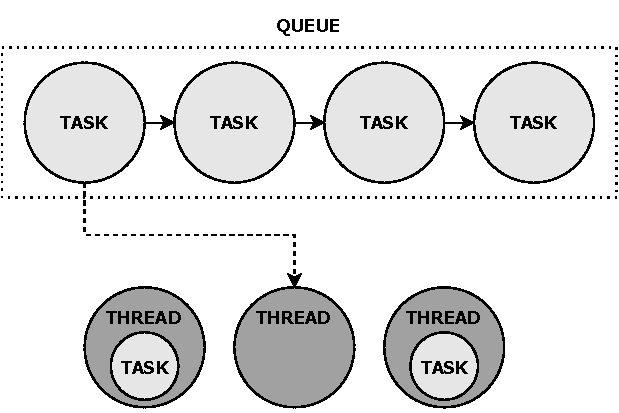
\includegraphics[width=0.55\textwidth]{patterns-work-pool.pdf}
    \caption{Wzorzec \textit{Work Pool}. Źródło: Opracowanie własne.}
    \label{fig:work-pool}
\end{figure}

\subsubsection{Wzorzec Pipeline}
Wzorzec \textit{Pipeline}, przedstawiony na rysunku \ref{fig:pipeline}, polega na potokowym przetwarzaniu danych. Nazywany jest również metodą producenta
i konsumenta. Strumień danych przekazywany jest do kolejnych wątków, które modyfikują oryginalny strumień.
Każdy z wątków wykonuje inny rodzaj obliczeń, które tworzą etapy potoku. Dane wyjściowe jednego etapu
stają się danymi wejściowymi kolejnego etapu. Stosowanie wzorca jest efektywne, jeśli czasy realizacji
poszczególnych etapów są~podobne \cite{wprowadzenie-do-obliczen-rownoleglych}.

\begin{figure}[H]
    \centering
	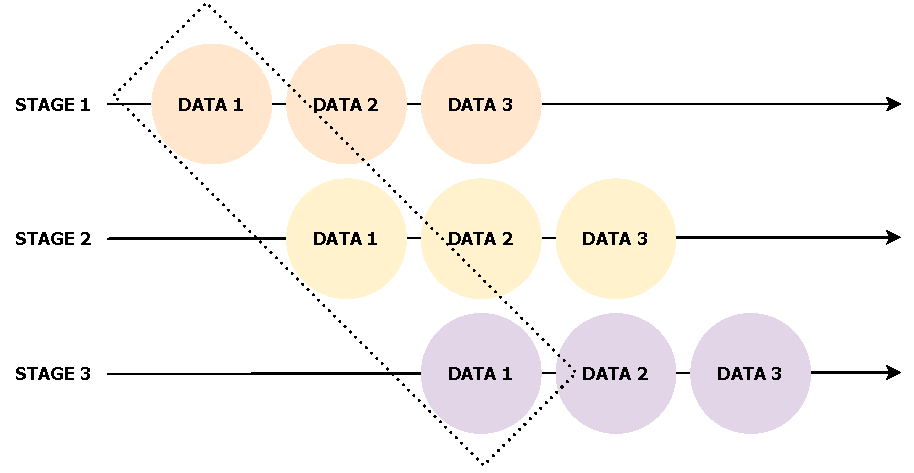
\includegraphics[width=0.75\textwidth]{patterns-pipeline.pdf}
    \caption{Wzorzec \textit{Pipeline}. Źródło: Opracowanie własne.}
    \label{fig:pipeline}
\end{figure}

\newpage

\section{Przegląd literatury}

Rozdział trzeci zawiera przegląd publikacji naukowych. Tematem omawianych prac są różne metody programowania równoległego stosowane
w algorytmach uczenia maszynowego.

\subsection{Równoległa konstrukcja algorytmu C4.5}

W artykule \cite{parallel-implementation-decision-tree} zostało przedstawionych kilka strategii konstrukcji algorytmów drzew decyzyjnych, które oparte są o techniki takie jak: równoległość zadań,
równoległość danych oraz równoległość hybrydowa. W pracy zaprezentowana została autorska implementacja równoległej konstrukcji drzewa
decyzyjnego algorytmem C4.5. Na zakończenie autorzy przedstawili wyniki działania algorytmu i postawili wstępne wnioski dotyczące jego działania.

Artykuł rozpoczyna się od zaprezentowania trudności, które pokazują, jak złożonym zadaniem jest implementacja równoległych
algorytmów do budowy drzew decyzyjnych. Wymienione zostają m.in. problemy z zastosowaniem statycznego, jak i dynamicznego przydzielania procesorów.
Nieregularny kształt drzewa, który określany jest dopiero w momencie działania programu, jest dużą przeszkodą do stosowania statycznej alokacji. Takie podejście prowadzi
najczęściej do nierównomiernego rozłożenia obciążenia. W przeciwnej sytuacji, gdy dane przetwarzane są przez dynamicznie przydzielane procesory, problemem staje się
konieczność zaimplementowania przekazywania danych. Współdzielenie danych jest wymagane, ponieważ część danych związanych z~rodzicami musi dostępna być również dla potomków.

Autorzy szczegółowo opisują różnice pomiędzy równoległością zadań, równoległością danych oraz równoległością hybrydową. Równoległość zadań określana jest
jako dynamiczne rozdzielanie węzłów decyzyjnych między procesory, w celu kontynuowania ich rozbudowy. Wadą takiego podejścia jest konieczność replikacji całego zbioru
treningowego lub, alternatywnie, zapewnienie częstej komunikacji pomiędzy procesorami. Równoległość danych przedstawiona jest jako wykonywanie tego samego zbioru instrukcji
algorytmu przez wszystkie zaangażowane procesory. Zbiór treningowy zostaje podzielony pionowo lub poziomo. Podział poziomy (horyzontalny) polega na na takim podziale danych między procesory, że
każdy z nich odpowiedzialny jest za inny zestaw przykładów ze zbioru treningowego. Podział pionowy (wertykalny) rozdziela przetwarzanie poszczególnych atrybutów między procesory.

Autorzy zwracają uwagę, że przetwarzanie z pionowym podziałem danych narażone jest na~wystąpienie nierównowagi obciążenia.
Równoległość hybrydowa scharakteryzowana jest jako połączenie równoległości zadań oraz danych. Dla węzłów, które muszą przetworzyć dużą liczbę przykładów, wykorzystywana
jest równoległość danych. W ten sposób unika się problemów związanych z nierównomiernym obciążeniem. W przypadku węzłów z przypisaną mniejszą liczbą przykładów
czas, potrzebny do komunikacji może być większy niż czas potrzebny do przetwarzania przykładów. Zastosowanie równoległości zadań w takie sytuacji pozwala uniknąć dysproporcji.

W kolejnej części artykułu przestawiona została implementacja równoległej konstrukcji drzewa decyzyjnego. Program został stworzony do wykonywania w środowisku pamięci
rozproszonej, w której każdy z procesorów ma~własną pamięć prywatną. Autorzy zaproponowali takie podejście, ponieważ ma ono rozwiązywać dwa problemy wspominane na
początku pracy: równoważenie obciążenia oraz konieczność przekazywania danych. Każdy z~procesorów ma~za~zadanie tworzyć własne listy atrybutów i klas na podstawie
przydzielonych podzbiorów przykładów. Wykorzystanie obydwu list jest kluczem do osiągnięcia efektywnego paralelizmu. Wpisy w liście klas zawierają etykietę klasy, indeks
globalny przykładu w zbiorze treningowym oraz~wskaźnik do węzła w drzewie, do którego należy dany przykład. Listy atrybutów również zawierają wpis dla każdego przykładu
z atrybutem, jak również indeks wskazujący na odpowiadający wpis w liście klas. Każdy procesor znajduje własne, najlepsze podziały lokalnego zbioru dla każdego atrybutu.
Następnie komunikuje się z pozostałymi procesorami, w celu ustalenia jednego, najlepszego podziału. Po podziale (utworzeniu węzła) następuje aktualizacja list atrybutów
przez każdy procesor, dokonana poprzez rozdzielenie atrybutów w zależności od wartości wybranego atrybutu dzielącego.

Zaprezentowane przez autorów wyniki określone są jako wstępne i wymagające udoskonaleń. Autorzy zdecydowali się jednak na wykorzystanie ich~do~przewidzenia oczekiwanego
zachowania algorytmu. Implementacja wykorzystuje takie same kryteria oceny jak stosowane w algorytmie C4.5, dlatego autorzy skupili się głównie na analizie czasu potrzebnego do
zbudowania drzewa. Do wszystkich testów wykorzystany był zestaw danych syntetycznych Agrawal, w którym każdy przykład ma dziewięć atrybutów (pięć ciągłych i~trzy dyskretne).

Z przedstawionych rezultatów testów wynika, że algorytm wykazał dobre wyniki przyspieszania. Twórcy artykułu przeprowadzili również testy mające na celu sprawdzenie skalowalności.
Jak w pierwszym przypadku, testy wykazały, że algorytm osiąga dobre wyniki skalowania.

\subsection{Zestawienie artykułów}

W literaturze można znaleźć wiele artykułów na temat metod programowania równoległego, które wykorzystywane są do optymalizacji algorytmów konstruujących drzewa decyzyjne. 
W pracach przedstawione są implementacje różnych wzorców programowania równoległego. W celu przybliżenia różnorodności oraz przedstawienia
dokładniejszego obrazu na temat wykorzystywanych wzorców i metod, artykuły zestawione zostały w tabeli. 

Tabela \ref{table:articles-parallel-decision-tree} zawiera odnośniki do tytułów artykułów, słowa kluczowe oraz krótki opis przybliżający tematykę poruszaną w każdym z artykułów.

    % \renewcommand{\arraystretch}{1.5}
    % \setlength{\tabcolsep}{0.07\textwidth}
    \begin{center}

        \begin{longtable}{| c | p{0.19\textwidth} | p{0.62\textwidth} |}
            \caption{Zestawienie artykułów poruszających tematykę\\ równoległości w algorytmach drzew decyzyjnych}
            \label{table:articles-parallel-decision-tree}
            \endfirsthead
            \endhead

            \hline
            
            \textbf{Artykuł} &\textbf{Słowa kluczowe} & \multicolumn{1}{|c|}{\textbf{Opis}}
            
            \\ \hline \hline 

            \cite{parallelization-of-decision-tree-al} &

            równoległość wewnątrzwęzłowa, równoległość międzywęzłowa &

            Autorzy przedstawili oraz porównali wydajność czterech metod do równoległej implementacji algorytmu C4.5.
            W~analizie uwzględniony został rodzaj danych wykorzystywanych do konstrukcji drzewa, który okazał
            się mieć duży wpływ na wyniki wydajności porównywanych metod. Wyszczególnione zostały trzy rodzaje
            techniki wewnątrzwęzłowej, które wykorzystują zrównoleglanie przetwarzania danych. Równolegle
            przetwarzane mogą być rekordy, atrybuty lub ich kombinacja (podejście hybrydowe). W technice międzywęzłowej
            równolegle przetwarzane są całe węzły -- wszystkie operacje, które muszą zostać przeprowadzone do stworzenia
            węzła, wykonywane są przez jeden wątek. \\
            
            \hline

            \cite{parallel-hoeffding-decision-tree} &

            węzły Hoeffdinga, architektura \textit{Master-Slave} &

            Autorzy artykułu zdecydowali się na zrównoleglanie tylko fragmentów algorytmu tj. szukania
            najlepszego atrybuty do podziału węzła. Zadania przydzielane przez główny procesor
            (\textit{master}) innym procesorom (\textit{slave}) polegają na~obliczenia zysku informacyjnego dla określonego
            atrybutu. Zastosowana architektura oraz zrównoleglanie tylko wyszukiwania atrybutów skutkuje
            jednak w niskiej skalowalności. Pomimo tego, testy wykazały, że przyspieszenie działania algorytmu
            jest dość efektywne. Dzięki zastosowaniu nierówności Hoeffdinga, do podziału drzewa nie muszą być
            używane wszystkie dane. Ma to dodatkowy wpływ na szybkość działania algorytmu. \\
            
            \hline

            \cite{parallel-algorithm-to-induce-decision-trees} &

            równoległość w węźle, duże zbiory danych &

            W artykule przedstawiono algorytm ParDTLT. Algorytm jest równoległą wersją algorytmu
            DTLT (ang. Decision Trees from Large Training sets), który nie wymaga ładowania w~całości wszystkich danych
            treningowych do pamięci komputera. ParDTLT oparty jest na idei sekwencyjnej budowy struktury
            drzewa oraz równoległym przetwarzaniu danych w każdym węźle. W danym czasie wszystkie procesory
            dostępne są dla jednego węzła. W węźle uprzywilejowanym tworzona jest kolejka atrybutów, dla
            których obliczany jest zrównoważony zysk informacji. Analiza kolejnych
            atrybutów przydzielane są procesorom do momentu, aż kolejka będzie pusta. Pozostałe węzły drzewa czekają, aż
            staną się węzłem uprzywilejowanym. Autorzy artykuły przeprowadzili testy algorytmu, które wykazały, że
            ParDTLT jest szybszy od algorytmów jak np. DTLT czy C4.5. \\

            \hline

            \cite{improved-id3-decision-tree} &

            pamięć \newline współdzielona, algorytm ID3 &

            Modyfikacjom został poddany algorytm ID3. Przedstawiono dwie różne implementacje wykorzystujące równoległość.
            Pierwsza polega na stworzeniu tylu wątków, ile istnieje atrybutów, dla których obliczony musi zostać
            przyrost informacji. Gdy atrybut dzielący zostanie odnaleziony, tworzony jest węzeł. Następnie ponownie
            tworzone są kolejne wątki, które przetwarzają atrybuty nowo powstałych węzłów. Dopiero gdy wszystkie wątki
            zakończą pracę, z dostarczonych wyników składane jest drzewo. Różnica w drugiej implementacji polega na 
            wykorzystaniu pamięci współdzielonej, dzięki czemu algorytm jest bardziej wydajny pamięciowo. 
            Węzeł główny jest współdzielony, dlatego każdy nowy węzeł może być tworzony, gdy tylko atrybut dzielący
            został odnaleziony. \\
            
            \hline
            
            \cite{research-parallel-map-reduce} &

            algorytm ID3, wzorzec \textit{Map-Reduce} &

            W pracy został zaprezentowany równoległy algorytm do budowy drzewa decyzyjnego, 
            który oparty jest na modelu \textit{Map-Reduce}. W pierwszej części, przedstawione zostały dwie główne metody podziału
            danych -- metoda dynamiczna i statyczna. Podobnie jak w \cite{parallel-implementation-decision-tree}, w ramach
            statycznej metody podziału danych wyróżniony został podział pionowy i poziomy. 
            Autorzy proponują zmodyfikowaną implementację algorytmu ID3 z wykorzystaniem biblioteki \textit{MapReduce}.
            Dane prezentowane są jako para (klucz, wartość). Etap ,,map'' polega na pionowym i poziomym podziale danych oraz generowaniu par klucz-wartość.
            Etap ,,reduce'' zawiera w sobie sumowanie częściowych wyników, odnalezieniu najlepszego atrybutu oraz
            przeprowadzaniu podziału. Omówiony na koniec przykład potwierdza, że tak skonstruowany algorytm jest w stanie
            w efektywny sposób przetwarzać duże ilości danych.\\

            \hline
 
        \end{longtable}

    \end{center}
\newpage

\section{Realizacja praktyczna}

Rozdział poświęcony jest opisowi różnych implementacji algorytmu ID3. W pracy nacisk położony jest na analizę
zastosowania równoległości w konstrukcjach drzew decyzyjnych, dlatego wybrano tylko jeden algorytm, który został
zaimplementowany na trzy różne sposoby. Pierwszy sposób to klasyczny, sekwencyjny algorytm ID3. Drugi sposób
wykorzystuje równoległość do obliczania zrównoważonego przyrostu informacji dla poszczególnych atrybutów.
Trzeci sposób opiera się na zastosowaniu równoległości podczas tworzenia całych węzłów drzewa decyzyjnego.
W rozdziale została również przedstawiona instrukcja uruchomienia programu, który zawiera wszystkie trzy
implementacje algorytmu.

\subsection{Implementacja}

Jako narzędzie został wybrany język programowania \textit{Java}, dlatego implementacja opiera się na podejściu
obiektowym. Język \textit{Java} oferuje wiele możliwości programowania współbieżnego i równoległego. W terminologii \textit{Java}
pojęcie wątek nabiera kolejnego znaczenia. Programista ma możliwość tworzenia wielu wątków, które zarządzane są
przez JVM (ang.~Java Virtual Machine) w celu równoległego wykonywania kodu. Inne dostępne mechanizmy to~synchronizacja,
blokady (ang. locks), semafory, interfejsy \textit{Callable} oraz \textit{Future}, zmienne typu \textit{atomic} czy framework \textit{Executor}.
Podczas fazy projektowania została przeprowadzona analiza, które z mechanizmów będą konieczne i pomocne
w implementacji. Ostatecznie w programie wykorzystane zostały głównie interfejsy \textit{Callable}, \textit{Future} oraz framework \textit{Executor}.

Kod został podzielony na pakiety (ang. package), które grupują klasy zgodnie~z~ich przeznaczeniem oraz funkcjonalnością. Zostało wydzielonych pięć pakietów:
\verb|classifier|, \verb|concurrent|, \verb|table|, \verb|tree| oraz \verb|utils|. Poniżej omówione zostaną tylko wybrane klasy, które są kluczowe z
punktu widzenia analizy równoległości oraz wydajności programu.

\subsubsection{Współdzielone fragmenty kodu}\label{common-code-blocks}

Jedną z głównych klas jest klasa \verb|DecisionTable|. Zawiera ona macierz \verb|String[][] table|, która przetrzymuje rekordy ze zbioru danych,
na podstawie których utworzone zostaje drzewo decyzyjne. W celu odnalezienia atrybutu dzielącego niezbędne jest wykonanie wielu obliczeń, które wymagają 
wstępnego uporządkowania danych np. odnalezienia indeksów w tabeli, w~których występują takie same wartości dla wybranego atrybutu $a_i$. 
Dostęp do części z uporządkowanych danych potrzebny jest kilkukrotnie w różnych fragmentach algorytmu. Z tego powodu zdecydowano o utworzeniu metadanych.
Koncepcja metadanych dotyczących zbioru danych opiera się na jednokrotnym przetworzeniu całej tabeli z rekordami i zgromadzeniu wszystkich niezbędnych
informacji, które w późniejszej fazie algorytmu będą koniecznie do ustalenia atrybutu dzielącego.

Do metadanych które zawiera klasa \verb|DecisionTable| należą następujące pola: \verb|Map<String,| \verb|Integer> decisionsFrequencies| -- mapa gromadzi informacje o częstości wystąpień
unikalnych wartości atrybutu decyzyjnego oraz \verb|AttributeValues[] attributesValues| -- tablica przetrzymująca instancje klasy \verb|AttributeValues|. Każdemu
atrybutowi $a_i$ (oprócz ostatniego, atrybutu decyzyjnego) odpowiada jedna instancja w tablicy \verb|attributesValues| przetrzymywana na miejscu o $i-1$ indeksie, czyli
takim samym jak indeks kolumny w tablicy \verb|table| zawierającej wszystkie wartości atrybutu $i$. Na przykładzie tabeli \ref{tab:decision-table} dla atrybutu $a_1$ zostałaby utworzona instancja klasy \verb|AttributeValue|, która umieszczona byłaby w tablicy
\verb|attributesValues| na miejscu o indeksie $0$.

Klasa \verb|AttributeValues| rozszerza klasę typu \verb|HashSet<AttributeValue>| a więc jest zbiorem obiektów typu \verb|AttributeValue|.
Zbiór zawiera tyle elementów, ile istnieje unikalnych wartości dla każdego atrybutu. Zadaniem klasy \verb|AttributeValue|, której szkielet przestawiony jest na
listingu \ref{lst:attribute-value-class}, jest przetrzymywanie informacji
powiązanych z jedną wartością atrybutu.

\begin{lstlisting}[language=java, caption=Skrócona implementacja klasy AttributeValue,frame=single,label={lst:attribute-value-class}]
public class AttributeValue {

    private final String value;
    private final Set<Integer> indices;
    private final Map<String, Integer>
                            decisionFrequenciesPerValue;

    public int getTotalFrequency() {...}

    public Collection<Integer> getFrequencies() {...}

    public AttributeValue(String value) {...}

    public void addIndex(int index) {...}

    public void addDecisionClass(String decisionClass) {...}
}
\end{lstlisting}
\newpage

Pole \verb|String value| przechowuje jedną, unikalną wartość atrybutu. Zbiór \verb|Set<Integer>| \verb|indices| zawiera indeksy, na których występują
wartości równe polu \verb|value|. Z kolei mapa \verb|Map<String, Integer> decisionFrequenciesPerValue| jako klucz przyjmuje wartość atrybutu decyzyjnego,
a jako wartość przechowuje częstość jego wystąpień, jednak tylko dla tych indeksów w tabeli \verb|table|, które zawierają się w zbiorze \verb|indices|.

Listing \ref{lst:attribute-value-example} przedstawia jak prezentowałyby się metadane dla atrybutu $a_1$ z tabeli \ref{tab:decision-table}.
Atrybut $a_1$ posiada dwie unikalne wartości: $v_{1,1}$ oraz $v_{1,2}$. Skutkuje to stworzeniem dwóch instancji klasy \verb|AttributeValue|.

\begin{lstlisting}[language=java, caption=Metadane na przykładzie atrybutu $a_1$ z tabeli \ref{tab:decision-table},frame=single,label={lst:attribute-value-example}]
System.out.println(attributesValues[0].toString());
# output:
# [ AttributeValue( value=v11,
#                   indices=[0, 2],
#                   decisionFrequenciesPerValue={c1=2} ),
#   AttributeValue( value=v12,
#                   indices=[1, 3, 4],
#                   decisionFrequenciesPerValue={c3=2, c2=1} ) ]
\end{lstlisting}
    
Tak przygotowane metadane zapewniają dostęp do wszystkich potrzebnych wartości, aby~obliczyć zrównoważony zysk informacji dla każdego
atrybutu znajdującego się w tabeli \verb|table|.

W pakiecie \verb|tree| znajduje się kolejna istotna klasa \verb|Node|. Klasa odwzorowuje węzeł drzewa decyzyjnego.
Wartość etykiety węzła \verb|String label| wskazuje numer atrybutu wybranego jako atrybut dzielący w węźle. Jeśli węzeł jest liściem, wówczas etykieta wskazuje na klasę decyzyjną.
Etykieta gałęzi \verb|String branchLabel| wskazuje na gałąź łączącą węzeł ze swoim rodzicem. Przechowuje więc ona jedną z wartości atrybutu dzielącego wybranego w węźle rodzica.
Jeśli węzeł jest korzeniem, wówczas etykieta gałęzi równa się \verb|null|. Lista węzłów \verb|List<Node> children| przechowuje listę potomków węzła. Dzięki niej, możliwe jest poruszanie się
po drzewie od korzenia w kierunku liści. Ostatnim polem zdefiniowanym w węźle jest tabela \verb|DecisionTable decisionTable|. Podczas tworzenia węzła korzenia tabela decyzyjna przechowuje
wszystkie rekordy, na podstawie których tworzone jest drzewo decyzyjne. Każdy podział drzewa skutkuje formowaniem się mniejszych tabel, które zawierają tylko część rekordów. W konsekwencji
każdemu węzłowi przypisana jest tabela zawierająca pewien podzbiór rekordów. Podzbiór zawiera te rekordy, których wartość dla atrybutu dzielącego węzeł rodzica jest równa etykiecie gałęzi, łączącej
potomka z rodzicem.

\subsubsection{Wykonanie sekwencyjne}
Wykorzystując specyfikę języka \textit{Java} można potraktować sekwencyjną implementacje algorytmu
jako bazę dla pozostałych dwóch, równoległych implementacji (mechanizm dziedziczenia).

Ujednoliconym warunkiem stopu tworzenia drzewa decyzyjnego jest sytuacja, gdy maksymalna wartość zrównoważonego
przyrostu informacji w węźle jest równa 0. Listing \ref{lst:sequential-tree} przedstawia metodę, która
umożliwia rozbudowę drzewa decyzyjnego do momentu, gdy warunek stopu zostanie spełniony. Na listingu widać, że budowa
drzewa odbywa się przy użyciu rekurencji \verb|createTree(child)|.
Obliczenia dla każdego atrybutu (od atrybutu o najmniejszym indeksie do atrybutu o najwyższym indeksie) jak i tworzenie węzłów potomków
(rozbudowując drzewo od lewej strony do prawej) wykonywane są sekwencyjnie. 

\begin{lstlisting}[language=java, caption=Rekurencyjne tworzenie drzewa decyzyjnego,frame=single,label={lst:sequential-tree}]
protected static void createTree(Node node) {
    DecisionTable table = node.getDecisionTable();

    if (table.getMaxGainRatio() == 0) {
        node.setLabel(table.getDecisionClass());
            return;
    }

    node.setLabel(table.getAttributeToDivideBy());

    for (AttributeValue metadata :
                        table.getValuesOfDividingAttribute()) {
        Node child = new Node(
            metadata.getValue(),
            table.getSubTable(metadata.getIndices())
        );
        node.addChild(child);
        createTree(child);
    }
}
\end{lstlisting}

\subsubsection{Równoległość na poziomie atrybutów}\label{executor-service}

Pierwsza równoległa implementacja polega na podziale zadań obliczenia zrównoważonego przyrostu informacji pomiędzy oddzielne wątki.
Jest to podejście które wykorzystuje równoległość danych. Dane dzielone są pionowo (wertykalnie).

Klasa \verb|ParallelDecisionTable| rozszerza klasę bazową \verb|DecisionTable|.
Została w niej nadpisana tylko jedna metoda \verb|int findAttributeToDivideBy()|, której celem jest odnalezienie atrybutu dzielącego.
W metodzie tworzona jest lista zadań obliczenia zrównoważonego przyrostu informacji \verb|List<ComputeGainRatioTask> taskList|.
Zadanie tworzone jest osobno dla każdego atrybutu i zdefiniowane jest w klasie \verb|ComputeGainRatioTask|, która implementuje interfejs \verb|Callable|.
Klasa w konstruktorze przyjmuje argumenty zawierające dane niezbędne do wykonania obliczeń:
indeks atrybutu, dla którego definiowane jest zadanie, lista częstości wystąpień
wartości klas decyzyjnych w tabeli decyzyjnej, liczba rekordów w tabeli decyzyjnej oraz zbiór obiektów typu \verb|AttributeValue|
tworzących metadane o przetwarzanym atrybucie. W klasie zdefiniowane są 4 prywatne metody, które służą obliczeniu wartości informacji \verb|double getInfo()|,
przyrostu informacji \verb|double getGain()|, wyznaczeniu informacji o podziale \verb|double getSplitInfo()|
oraz obliczeniu zrównoważonego przyrostu informacji \verb|getGainRatio()|. Jedna metoda publiczna \verb|GainRatioResult call()|, której
implementacja wymuszona jest przez interfejs \verb|Callable|, umożliwia start wykonywania zadania przez wątek, któremu zostało ono przydzielone.

Klasa \verb|ExecutorService| udostępnia metodę przyjmującą jako parametr listę zadań, które mają zostać wykonane równolegle. Podczas tworzenia instancji
klasy \verb|ExecutorService| należy zdefiniować liczbę wątków, które będą przetwarzać listę zadań. Implementacja opiera się na~wzorcu \textit{Work Pool} \ref{work-pool}.
Zadania z listy przekazywane są wolnym wątkom do momentu, aż~wszystkie zadania zostaną rozdzielone i wykonane. Istotny jest fakt, iż dostęp do rezultatów
jest dostępny dopiero wtedy, gdy wszystkie wątki zakończą prace. Taki mechanizm nazywany jest blokującym. W momencie, gdy wszystkie wyniki zgromadzone
zostaną w formie listy, wybierany jest ten atrybut, dla którego obliczony zrównoważony przyrost informacji jest największy. W ten sposób odnajdywany jest atrybut dzielący.

\subsubsection{Równoległość na poziomie węzłów}

Różnica pomiędzy pierwszą a drugą równoległą implementacją, polega na zmianie definicji zadania równoległego. W tym przypadku, zadanie polega na stworzeniu jednego
węzła. Zadanie zdefiniowane jest w klasie \verb|CreateNodeTask|, która również implementuje interface \verb|Callable|. Klasa zawiera tylko jedną metodę
\verb|Node call()|, jednak większość równoległej implementacji zawiera się w klasie \verb|ParallelNodesDecisionTree|, która rozszerza klasę \verb|DecisionTree|.
W klasie tej została nadpisana jedna metoda \verb|createTree(Node node)|. Warunek zatrzymania tworzenia drzewa decyzyjnego pozostaje bez zmian. Różnice w
implementacji widoczne są podczas tworzenia węzłów potomnych.

Lista zawiera zadania utworzenia każdego z węzłów potomnych (bez kolejnego pokolenia potomków). Lista zadań tworzona jest oddzielnie
dla każdego węzła rodzicielskiego.

\begin{lstlisting}[language=java, caption=Lista zadań równoległego tworzenia węzłów,frame=single,label={lst:create-node-parallel}]
List<Callable<Node>> taskList = new ArrayList<>();

for (AttributeValue attributeValue :
                        table.getValuesOfDividingAttribute()) {
    CreateNodeTask createNodeTask = CreateNodeTask.builder()
            .decisionTable(table)
            .attributeValue(attributeValue)
            .build();

    taskList.add(createNodeTask);
}
\end{lstlisting}

Podobnie jak przy równoległym przetwarzaniu na poziomie atrybutów, został wykorzystany wzorzec Work-Pool.
Mechanizm blokujący ponownie wstrzymuje przejście do kolejnej fazy algorytmu do momentu, gdy wszyscy potomkowie rodzica nie zostaną stworzeni
i dodani do listy \verb|children|. Po zakończeniu działania współbieżnej części kodu jako pierwszy zostaje wybrany potomek, który znajduje się
na pierwszym miejscu listy \verb|childern|. Na tym etapie rozwój drzewa przenoszony jest na niższy poziom. Potomek staje się rodzicem
i procedura tworzenia listy zadań powtarza się. Drzewo rozwijane jest w lewo tak długo, aż któryś z węzłów potomnych stanie się liściem.
Wówczas algorytm rekurencyjnie powraca do pominiętych węzłów w celu stworzenia ich potomków.

\subsection{Uruchamianie programu}

Program został napisany w języku \textit{Java} w wydaniu 11, dlatego aby go uruchomić, konieczna jest instalacja środowiska \textit{Java Runtime Environment (JRE)}
w wersji 11 lub wyższej. Wszystkie pliki z kodem źródłowym zostały skompilowane i na ich podstawie stworzony został wykonywalny plik archiwum \textit{Java JAR}.

Program został sparametryzowany tak, aby mógł zostać uruchomiony w każdym wariancie implementacji algorytmu ID3. Niezbędne jest również
podanie ścieżki do pliku ze zbiorem danych. Argumenty pozwalają na ustawianie następujących wartości:

{\renewcommand\labelitemi{}
\begin{itemize}
    \item \verb|--data-set| -- ścieżka do pliku ze zbiorem danych,
    \item \verb|--delimiter| -- separator wartości w zbiorze danych,
    \item \verb|--output-file| -- ścieżka do pliku, gdzie zapisane zostaną dane o wydajności wykonania programu potrzebne do analizy,
    \item \verb|--threads| -- liczbę użytych wątków,
    \item \verb|--test-ratio| -- udział procentowy danych losowo wybieranych do zbioru testowego,
    \item \verb|--train-ratio| -- udział procentowy danych losowo wybieranych do zbioru treningowego, wartość wraz z \verb|--test-ratio| muszą być równe 1,
    \item \verb|--type| -- wersja algorytmu.
\end{itemize}}

Aby uruchomić program w wersji sekwencyjnej argument \verb|--type| należy ustawić na wartość \verb|SEQUENTIAL|.
W celu zastosowania równoległości na poziomie atrybutów, użytkownik musi podać wartość \verb|PARALLEL_ATTRIBUTES|.
Ustawienie argumentu na wartość \verb|PARALLEL_NODES| spowoduje uruchomienia algorytmu w wersji z równoległością węzłów.

\begin{lstlisting}[caption=Przykładowe uruchomienie programu,frame=single]
    java -jar concurrent-id3.jar
        --data-set ./resources/data.csv\
        --delimiter ,\
        --output-file ./results.txt\
        --threads 5\
        --test-ratio 0.1\
        --train-ratio 0.9\
        --type PARALLEL_NODES
\end{lstlisting}

\newpage
\section{Analiza wyników}

Rozdział piąty zawiera opis analizy algorytmów pod kątem ich wydajności. Poruszone zostały
tematy związane z czasem trwania poszczególnych wykonań algorytmu, zużyciem pamięci RAM, pamięci
przydzielonej procesowi i liczbę wykorzystanych wątków. Analiza oparta jest na danych zgromadzonych
dzięki przeprowadzonym testom. Wyniki pomiarów zostały przedstawione w formie
wykresów stworzonych przy użyciu języka \textit{Python} oraz biblioteki \textit{Plotnine}, która umożliwia
korzystanie z pakietu \textit{ggplot2}.

\subsection{Środowisko testowe}
Większość testów zostało przeprowadzonych na komputerze z 4 rdzeniowym procesorem Intel Core i7-7700HQ
z 16GB pamięci RAM. Dodatkowo, do przeprowadzania jednego typu testów, użyto komputera z 4 rdzeniowym procesorem AMD
Ryzen 5 2500U z 8 GB pamięci RAM.

Podczas przeprowadzania testów wydajnościowych istotne jest zachowanie podobnych warunków środowiska testowego.
Nie jest możliwe całkowite wyłączenie innych aplikacji, ponieważ o działaniu wielu z nich decyduje
system operacyjny. Jednakże w celu minimalizacji obciążenia procesora innymi procesami, wszystkie możliwe
do zatrzymania programy zostały wyłączone.

Dodatkową techniką, która miała na celu zmniejszenie wpływu zewnętrznych czynników na rezultaty testów,
było zastosowanie uśredniania wyników. Dla każdej konfiguracji parametrów program został uruchomiony kilkukrotnie.
Zebrane wyniki zostały uśrednione, aby~wygenerowane wykresy stały się przez to bardzo wiarygodne.
Ręczne uruchamianie programu z~wiersza poleceń jest mało optymalne, dlatego cały proces zbierania rezultatów testów
został zautomatyzowany. W celu wielokrotnego uruchomienia programu dla różnych parametrów, zostały utworzone
skrypty w języku \textit{Bash}.

\subsection{Kryteria testów wydajnościowych}

W przypadku implementacji algorytmu ID3, głównym celem zastosowania przetwarzania wielowątkowego było
skrócenie czasu budowy drzewa decyzyjnego. Analizowanie wydajności w pierwszej kolejności wymaga ustalenia, czy stworzony
program jest w stanie dostarczać poprawne wyniki.
W celu walidacji poprawności kluczowych elementów implementacji, program został przetestowany za
pomocą testów jednostkowych. Klasy zawierające logikę, która wpływa na strukturę drzewa, zostały przetestowane
na danych, dla których znany był poprawny kształt drzewa. Dzięki uzyskaniu pozytywnych wyników
testowania algorytmu pod względem poprawności, podczas analizy kluczowej dla tematu pracy, cała
uwaga została skupiona już tylko na badaniu wydajności.
W dalszej części rozdziału omówione zostały kryteria testów przeprowadzonych pod kątem wydajności
poszczególnych implementacji algorytmu ID3.

\subsubsection{Rozmiar danych}
Czynnikiem, który ma istotny wypływ na czas konstruowania klasyfikatora jest rozmiar
danych. Podczas implementowania algorytmów, często korzysta się z małych zbiorów danych,
które ułatwiają testowanie ich poprawności. Dopiero w momencie, gdy algorytm zostanie
uruchomiony dla rzeczywistych danych, istnieje możliwość sprawdzenia, czy program jest w stanie
efektywnie przetwarzać dane i dostarczyć ostateczne rozwiązanie. 
Rysunek \ref{fig:analysis} przedstawia, jak zmienia się całkowity czas potrzebny na konstrukcje
klasyfikatora, w zależności od liczby rekordów w zbiorze danych. Na wykresie ujęto trzy rodzaje algorytmu:
wersja sekwencyjna, zrównoleglanie atrybutów oraz zrównoleglanie węzłów.

\begin{figure}[H]
    \centering
	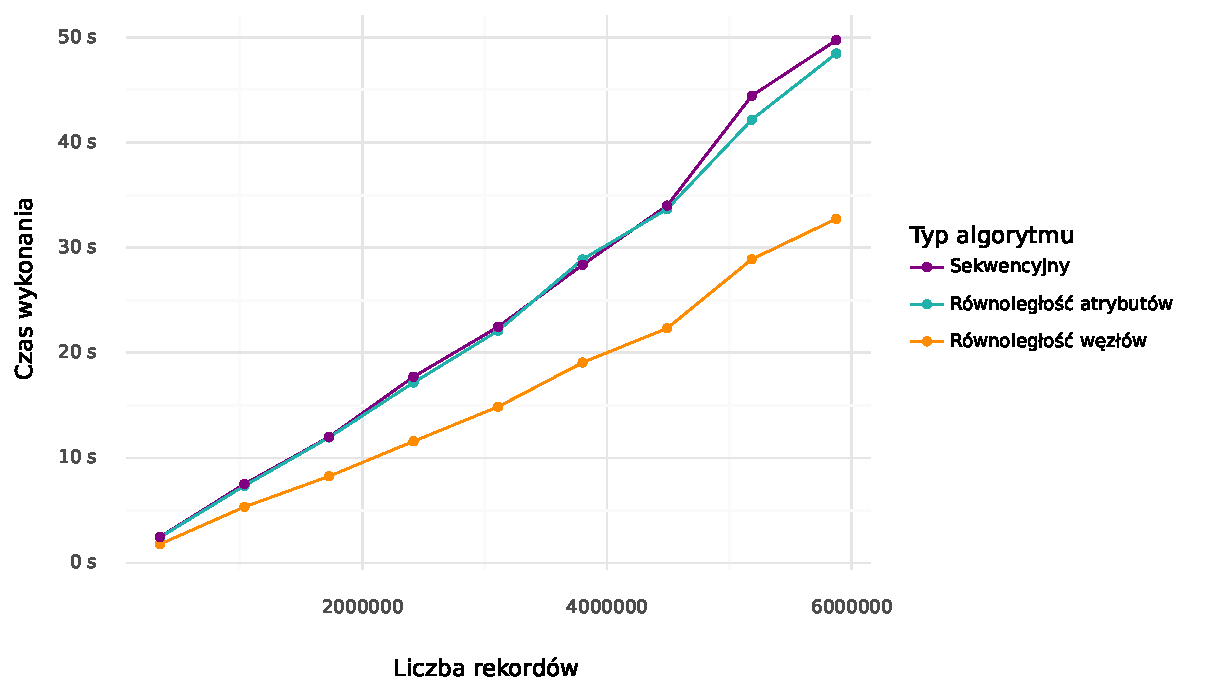
\includegraphics[width=0.9\textwidth]{analysis.pdf}
    \caption{Zależność czasu od liczby rekordów.\\Źródło: Opracowanie własne.}
    \label{fig:analysis}
\end{figure}

Przy niewielkiej liczbie rekordów czas trwania wszystkich trzech implementacji algorytmu ID3 jest prawie identyczny.
Wraz z rosnącą liczbą rekordów, najlepsze rezultaty osiąga algorytm, gdzie zastosowano równoległość węzłów. Zastosowanie
algorytmu z równoległością atrybutów nie przynosi znaczących korzyści. Czas budowy klasyfikatora, bez względu na liczbę rekordów,
praktycznie nie różni się od czasu osiąganego dla implementacji sekwencyjnej. 

Po przeanalizowaniu rozwiązania z równoległym przetwarzaniem atrybutów, zostały wyciągnięte następujące wnioski.
Implementacja jest mało efektywna bez względu na rodzaj i wielkość zbioru danych. Prawdopodobną przyczyną niskiej
wydajności implementacji jest zastosowanie konceptu metadanych. Jak opisano w rozdziale \ref{common-code-blocks}, celem tworzenia
metadanych było zredukowanie liczby powtarzanych obliczeń. Wiąże się to z tym, że najbardziej obciążające obliczenia
dokonywane są w momencie tworzenia metadanych. Z tego powodu, obliczanie zrównoważonego przyrostu informacji dla każdego
atrybutu jest działaniem mało złożonym obliczeniowo. Koszt powoływania do życia wątków oraz obsługi równoległości jest większy
niż korzyść płynąca z równoległego przetwarzania atrybutów.

Inaczej sytuacja prezentuje się w przypadku równoległego przetwarzania węzłów. Tutaj równolegle tworzone są całe węzły. Operacje, które wykonywane są
podczas tworzenia węzła to tworzenie metadanych jak i obliczanie zrównoważonych zysków informacji. Wspólnie, działania wymagają
sporo mocy obliczeniowej i dlatego zastosowanie równoległości jest uzasadnione. Takie rozwiązanie sprawia, że implementacja jest skuteczna.

Sytuacja odwraca się w przypadku przetwarzania małych zbiorów danych. Niewielkie bloki danych nie wymagają dużej mocy obliczeniowej
nawet w przypadku tworzenia metadanych.

\begin{figure}[H]
    \centering
	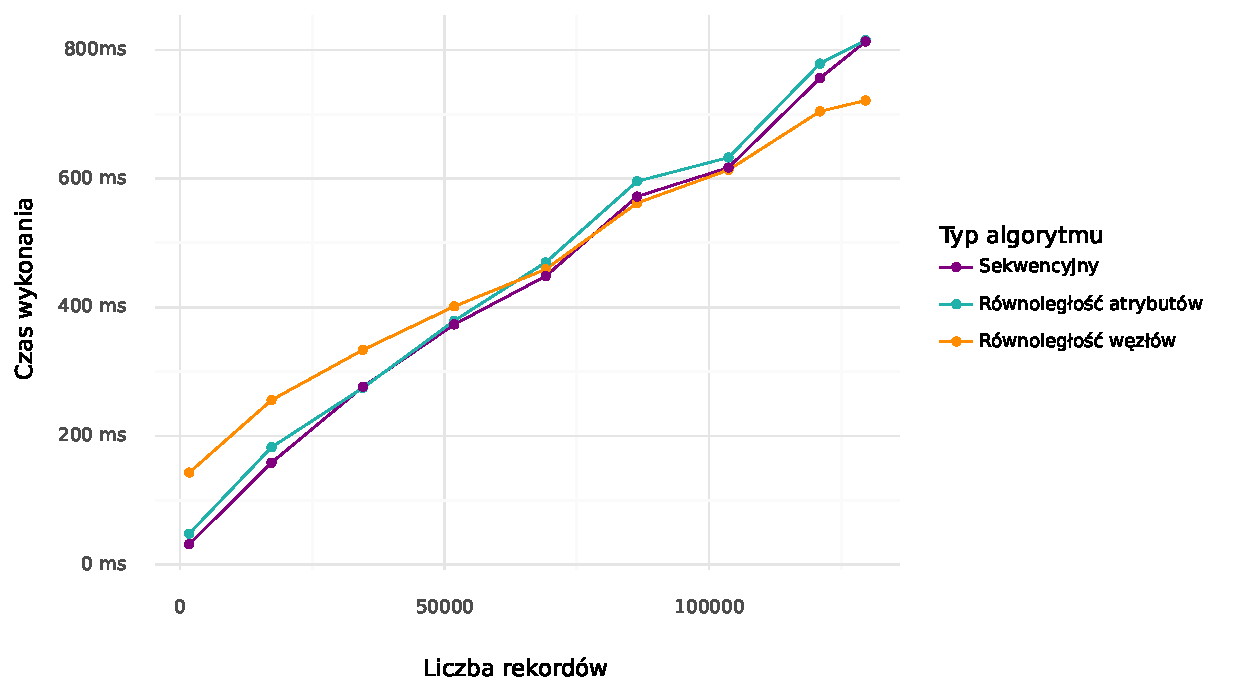
\includegraphics[width=0.9\textwidth]{analysis-start.pdf}
    \caption{Zależność czasu od liczby rekordów przy małym\\obciążeniu procesora. Źródło: Opracowanie własne.}
    \label{fig:analysis-start}
\end{figure}

Rysunek \ref{fig:analysis-start} ponownie prezentuje zależność czasu wykonania od
liczby rekordów, jednak na~przykładzie zbiorów danych o małych rozmiarach. Liczba rekordów wacha się od 120 do~140000. 
Im mniej rekordów jest przetwarzanych, tym bardziej efektywny jest algorytm sekwencyjny.

Kolejną składową wpływającą na wielkość zbioru danych jest liczba atrybutów. Im więcej atrybutów posiada
rekord, tym więcej obliczeń zrównoważonego przyrostu informacji musi zostać wykonanych na poziomie każdego węzła.
Rysunek \ref{fig:analysis-attributes} przedstawia zależność czasu wykonania algorytmu od rosnącej liczby atrybutów.
Zaprezentowane wyniki zostały utworzone na podstawie zbiorów danych, z których każdy zawierał po 3000 rekordów.

\begin{figure}[H]
    \centering
	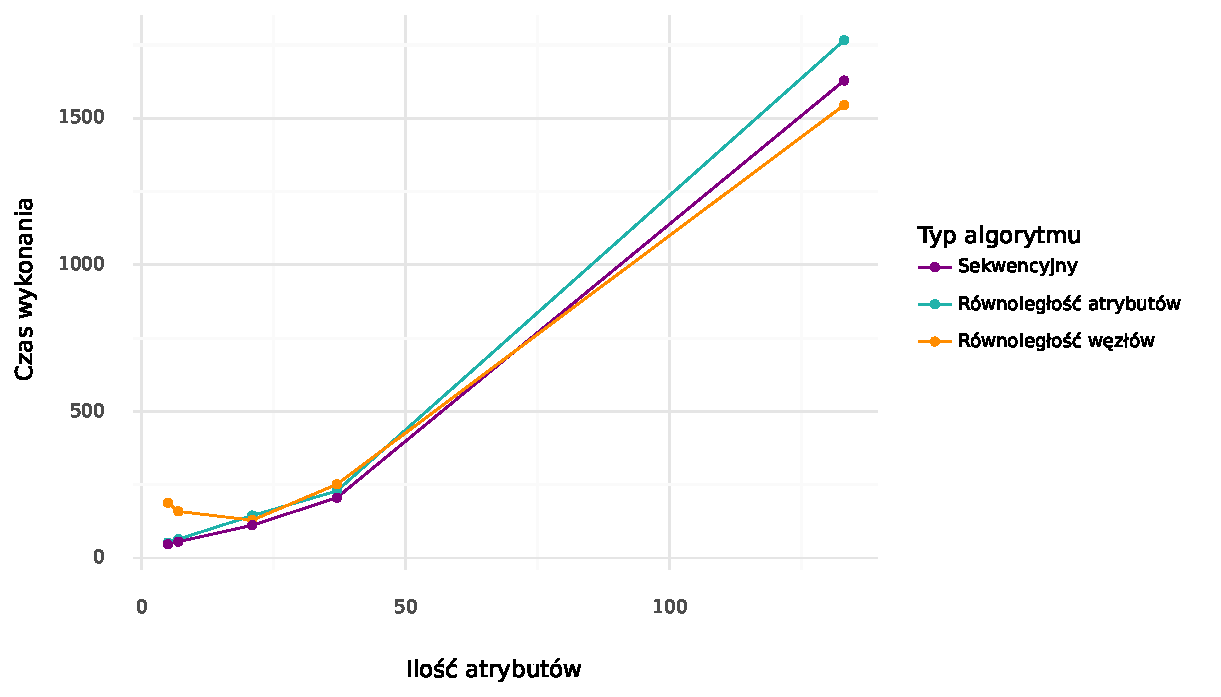
\includegraphics[width=0.9\textwidth]{analysis-attributes.pdf}
    \caption{Zależność czasu od liczby atrybutów.\\Źródło: Opracowanie własne.}
    \label{fig:analysis-attributes}
\end{figure}

Podobnie jak w przypadku zwiększania liczby rekordów, dla niewielkiej liczby atrybutów, algorytm ze
zrównolegleniem węzłów okazał się być mniej efektywny niż pozostałe. Moment wyrównania
przypada na około 20 atrybutów. Przy stopniowym zwiększaniu liczby atrybutów widać, że
zachodzą różnice w stosunku do zwiększania liczby rekordów.
Na wykresie można zauważyć, że wydajność algorytmów równoległych
nie ulega wyraźniej poprawie. Przy 130 atrybutach czas wykonania programu, gdzie równolegle przetwarzane są węzły
jest niewiele lepszy od pozostałych. W celu wyciągnięcia wniosków, konieczne było sprawdzenie jak kształtuje się
wykres dla większej liczby atrybutów. Znalezienie zbiorów danych nadających się do~testowania algorytmu ID3, w których liczba
atrybutów będzie wzrastała proporcjonalnie, nie jest łatwym zadaniem. Z tego powodu, wykres na rysunku \ref{fig:analysis-attributes-bar-plot} przedstawia zależności tylko dla
jednego, największego pod względem liczby atrybutów zbioru danych, który udało się uzyskać do celów badania (13 200 atrybutów).

\begin{figure}[H]
    \centering
	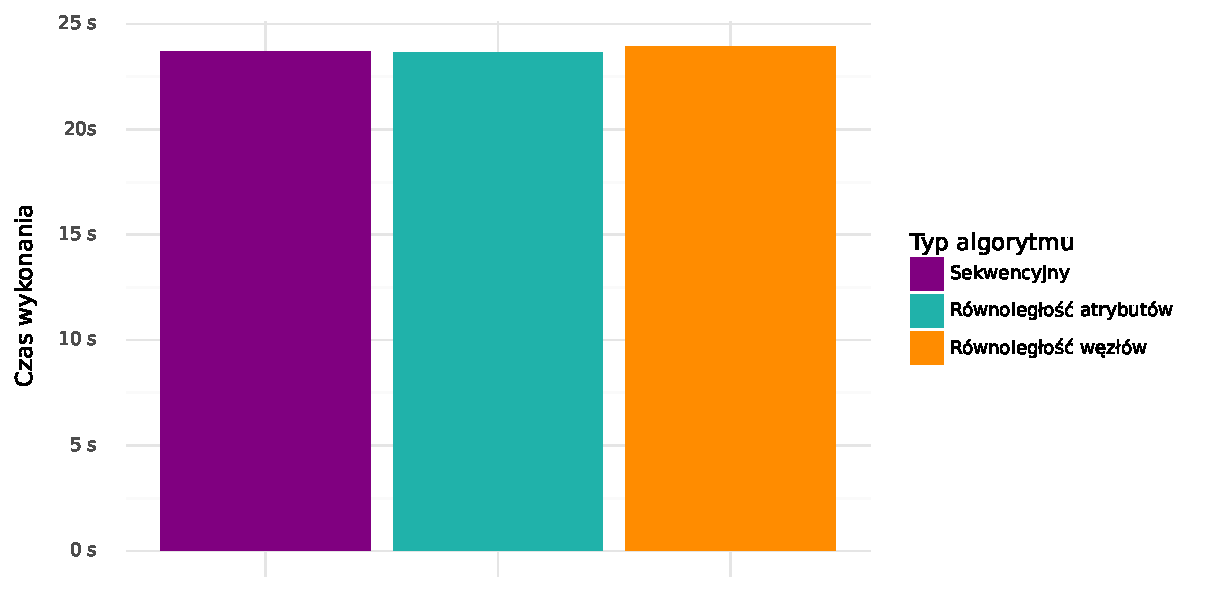
\includegraphics[width=0.9\textwidth]{analysis-attributes-bar-plot.pdf}
    \caption{Czas wykonania programu dla danych\\ o 13 200 atrybutach. Źródło: Opracowanie własne.}
    \label{fig:analysis-attributes-bar-plot}
\end{figure}

Wykres na rysunku \ref{fig:analysis-attributes-bar-plot} daje podstawy do stwierdzenia, że żadna ze stworzonych implementacji równoległych nie jest optymalna,
gdy obciążenie procesora spowodowane jest dużą liczbą atrybutów.

\subsubsection{Ilość pamięci RAM oraz pamięci Heap Space}

Kolejnym czynnikiem ważnym podczas przeprowadzania analizy wydajności programu jest dostępna pamięć.
Pamięć operacyjna RAM pełni funkcje pośrednika pomiędzy pamięcią tymczasową a dyskami twardymi.
W pamięci tej przechowywane są m.in.: informacje na temat działających programów. Procesor wykorzystuje informacje
przechowywane w pamięci RAM w celu zarządzania procesami.
Większa ilość pamięci RAM korzystnie wpływa na szybkość i płynność działania programów. 
Z powodu braku możliwości zwiększenia ilości pamięci RAM w komputerze, na którym przeprowadzane były testy, zdecydowano, że
przeprowadzona zostanie serie testów na oddzielnym sprzęcie o innych parametrach. Program został uruchomiony
dla jednakowego zbioru danych na dwóch różnych komputerach z dostępnymi 8GB oraz 16 GM pamięci RAM.
Wykres \ref{fig:analysis-start} został rozszerzony o rezultaty zgromadzone podczas testów na komputerze z 8GB pamięci RAM.
Wyniki zaprezentowane są na rysunku \ref{fig:analysis-ram}.

\begin{figure}[H]
    \centering
	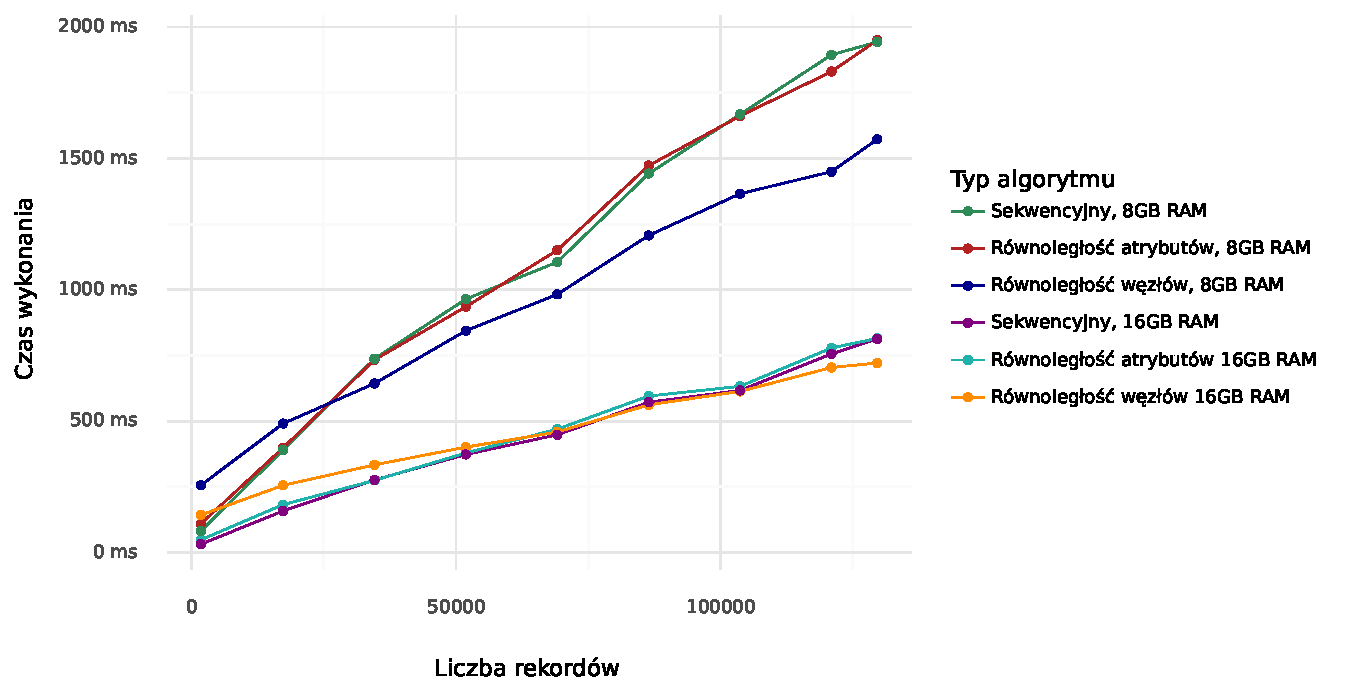
\includegraphics[width=0.9\textwidth]{analysis-ram.pdf}
    \caption{Zależność czasu od liczby rekordów i dostępnej\\pamięci RAM. Źródło: Opracowanie własne.}
    \label{fig:analysis-ram}
\end{figure}

Mniejsza ilość pamięci RAM znacząco wpływa na czas potrzebny do stworzenia klasyfikatora.
Prawie każde wykonanie algorytmu na komputerze z dostępnymi 16GB pamięci RAM było szybsze niż
jakiekolwiek wykonanie algorytmu na komputerze z 8GB pamięci RAM.

Czasy wykonań poszczególnych implementacji algorytmu ID3, są bardziej zróżnicowane dla rezultatów
osiągniętych na komputerze z 8GB pamięci.
Nie jest to jednak dowód na to, że zrównoleglanie węzłów jest bardziej efektywne
na komputerze o słabszych parametrach. Mniejsza ilość pamięci RAM skutkuje dłuższym
czasem wykonania algorytmu. Jak pokazano w pierwszej części analizy, stosowanie równoległości jest skuteczniejsze,
gdy procesor jest bardziej obciążony. Z tego powodu, wykres sprawia wrażenie, że algorytm wykonywany na~słabszym
sprzęcie działa bardziej efektywnie.
Dla każdego komputera można ustalić moment, w którym stosowanie równoległości przynosi korzyści. Jest to moment
przecięcia się lini odpowiadającej wykonaniu równoległemu z linią odpowiadającą wykonaniom sekwencyjnym.
Dla słabszego komputera moment ten przypada na około 120 tys. rekordów. Dla mocniejszego komputera
jest to około 5 tys. rekordów.

Kolejnym typem pamięci uwzględnionym podczas analizy wydajności jest pamięć nazywana stertą (ang. Heap Space). Jest to wydzielona
część pamięci RAM, która przydzielona jest maszynie wirtualnej \textit{Javy} w czasie jej startu.
Podczas uruchomiania programu, napisanego w języku \textit{Java}, istnieje możliwość konfiguracji ilości
pamięci RAM przydzielonej maszynie wirtualnej. Parametr \verb|-Xmx| umożliwia konfigurację maksymalnej
wartości sterty (ang. Heap Size). Przykładowo dodając parametr \verb|-Xmx4096m|
maksymalna wartość \textit{Heap Size} wynosi 4096 megabajtów. Powiększanie \textit{Heap Size} ma sens, jeśli do pamięci programu
ładowane są bardzo duże ilości danych. Jeśli wartość pozostanie na niskim poziomie, wówczas pamięć zostaje przepełniona, w wyniku czego
program zostaje przerwany z powodu błędu typu \verb|java.lang.OutOfMemoryError|.

\begin{figure}[H]
    \centering
	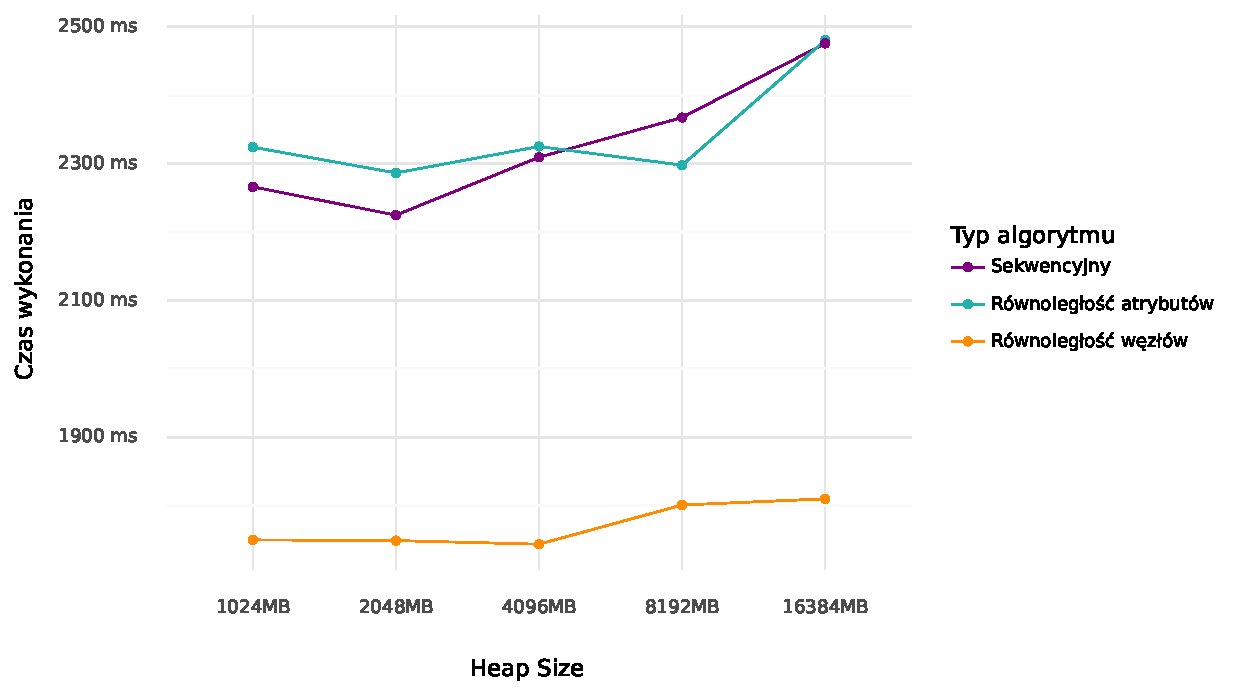
\includegraphics[width=0.9\textwidth]{analysis-heap-size.pdf}
    \caption{Zależność czasu od wartości \textit{Heap Size}.\\Źródło: Opracowanie własne.}
    \label{fig:analysis-heap-size}
\end{figure}

W oparciu o rysunek \ref{fig:analysis-heap-size} można stwierdzić, że w odróżnieniu do pamięci RAM,
zwiększanie wartości \textit{Heap Size} nie wpływa bezpośrednio na poprawę wydajności którejkolwiek implementacji algorytmu.
Pomiary zostały wykonane dla jednego zbioru danych, dla którego bez problemu można było uruchomić algorytm nawet
przy niskiej wartości \textit{Heap Size}. Wraz ze wzrostem wartości \textit{Heap Size} nastąpiło nieznaczne pogorszenie efektywności działania programu. 
Może ono wynikać z tego, że uruchomianie maszyny wirtualnej \textit{Javy} z większą ilością przydzielonej pamięci, jest bardziej czasochłonnym procesem.

\subsubsection{Liczba wątków}
Ostatnim przeanalizowanym zagadnieniem był wpływ liczby tworzonych wątków na czas trwania
pracy programu. Podczas tej analizy, pojęcie wątek używane jest w kontekście wątków
tworzonych w ramach maszyny wirtualnej \textit{Javy}. Każdy wątek tworzony przez \textit{JVM} związany jest
z klasą \verb|java.lang.Thread|. Tworzenie instancji wymienionej klasy rozpoczyna cykl życia wątku.
Dopuszczalne stany, w których może znajdować się wątek to m.in.: \verb|RUNNABLE|, 
\verb|BLOCKED| czy \verb|WAITING|. Programista może zarządzać liczbą wątków poprzez jawne tworzenie instancji
klasy \verb|Thread| lub też może skorzystać z interfejsu \verb|Executor|, w ramach którego tworzone są pule wątków.

Rysunek \ref{fig:analysis-threads} przedstawia wyniki testów przeprowadzonych pod kątem zmiennej
liczby przydzielanych wątków.

\begin{figure}[H]
    \centering
	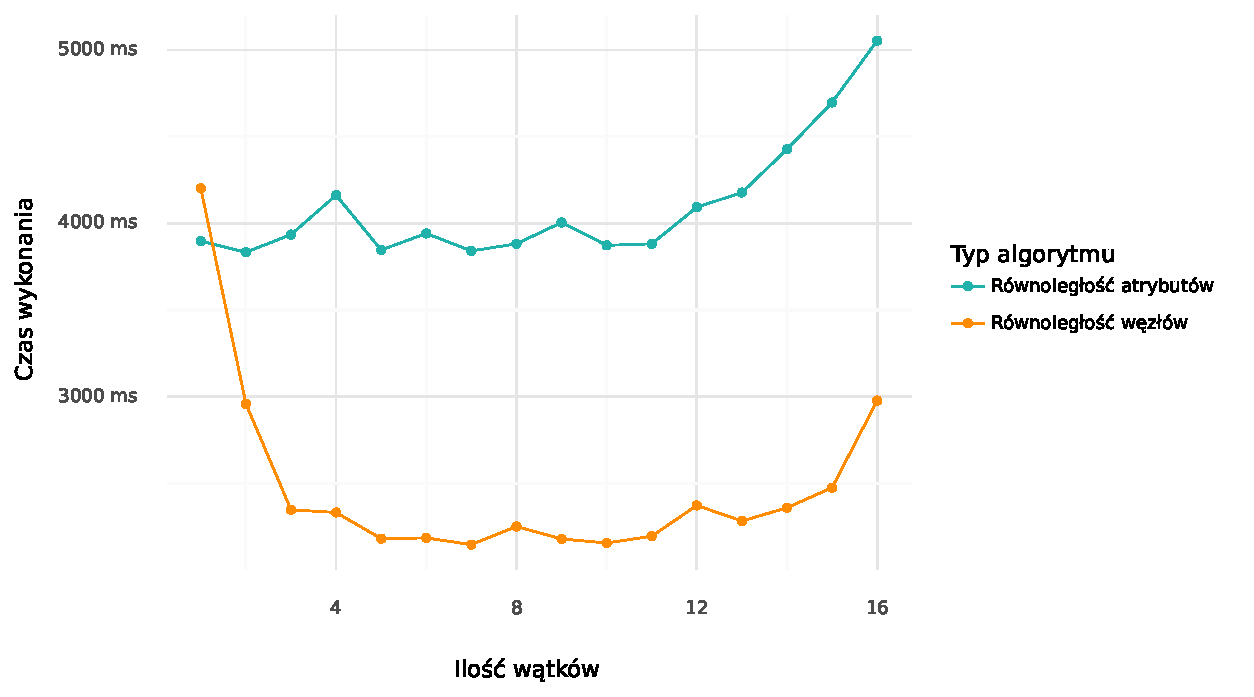
\includegraphics[width=0.9\textwidth]{analysis-threads.pdf}
    \caption{Zależność czasu od liczby przydzielonych wątków.\\Źródło: Opracowanie własne.}
    \label{fig:analysis-threads}
\end{figure}

Liczba wątków, którą należy użyć w programie \textit{Java} zależy od wielu czynników. Największe znaczenie
mają zasoby sprzętowe, charakter oraz obciążenie programu.
Zaleca się stosowanie liczby wątków równej lub trochę większej od liczby dostępnych rdzeni logicznych.
Komputer, na którym przeprowadzano testy posiada 4 rdzenie fizyczne co w konsekwencji daje do
dyspozycji 8 rdzeni logicznych. Na grafice \ref{fig:analysis-threads} widać, że
zbyt mała liczba wątków istotnie wydłuża czas pracy programu.
Podobnie zbyt duża liczba wątków opóźnia moment zakończenia pracy programu. Przyczyną takiej tendencji, 
są ograniczone zasoby systemu operacyjnego, które umożliwiają
efektywne przetwarzanie tylko ograniczonej liczby równoległych operacji. Powoływanie do życia nowego wątku
jest kosztowną operacją, dlatego tworzenie wątków w~zbyt dużej jak i zbyt małej liczbie, negatywnie wpływa
na efektywność programu.

\subsection{Zaistniałe problemy}
Pierwotnie program został zaimplementowany z wykorzystaniem uproszczeń jakie oferuje język \textit{Java} w wersji 11
jak np. strumienie (\textit{Java Stream API}). Interfejs strumieni umożliwia tworzenie
bardziej spójnego i czytelnego kodu. Korzystanie z udogodnień może wiązać się jednak ze skutkami ubocznymi.
Obliczenia na dużych zbiorach danych znacznie obciążają procesor, co skutkuje zwiększeniem czasu
potrzebnego na wykonanie programu. Z tego powodu, w celu poprawy wydajności wprowadzono poprawki
takie jak zastąpienie list przez tablice (tam, gdzie to możliwe), a także rezygnacja
z użycia strumieni i zamiana ich na pętle for.

Kolejnym problemem, który został zaobserwowany była gwałtownie rosnąca ilość wykorzystanego \textit{Heap Space}.
Język \textit{Java} oferuje mechanizm usuwania nieużytków \textit{Garbage Collection}. Oznacza to, że programista nie zarządza
samodzielnie przydzielaniem jak i zwalnianiem pamięci. Za te czynności odpowiedzialny jest program nazywany \textit{Garbage Collector}.
Podstawowe zadania programu to alokacja pamięci oraz odzyskiwanie jej dzięki usuwaniu obiektów, do których nie istnieją już referencje.
Pomimo tego, iż programista nie jest bezpośrednio odpowiedzialny za zarządzanie pamięcią, istnieje kilka typów błędów w
implementacji, które mogą powodować wycieki pamięci (ang. Memory Leaks). Wycieki powodują przepełnienie pamięci,
co skutkuje przerwaniem pracy programu.
Dzięki użyciu narzędzi takich jak \textit{Java~VisualVM}~możliwe jest generowanie wykresów wykorzystania stosu
w trakcie działania programu.
W celu rozwiązania problemu, podjęte zostały próby odnalezienia ewentualnych miejsc wycieków pamięci.
Wykresy analizy wykonanej narzędziem \textit{Java VisualVM} pokazały, że ilość zaalokowanej pamięci rosła wraz
z czasem trwania programu, a \textit{Garbage Collector} nie miał możliwości zwalniania jej dostatecznie szybko. 
Najprawdopodobniej kluczową rolę w zaistniałym problemie odgrywa wykorzystanie rekurencji, która nie jest optymalna pod względem
zajmowanej pamięci. Dodatkowym czynnikiem może być konieczność ładowania do pamięci programu dużych zbiorów danych.
Próbą zmniejszenia zużycia pamięci na stosie było zaimplementowanie współdzielenia danych. Zamiast duplikacji części rekordów,
przekazywanych do węzłów potomnych, przekazywane były tylko numery indeksów, które dotyczyły wybranego węzła.
Niestety zaimplementowane poprawki nie przyniosły pozytywnych rezultatów.
Podejście dostarczania danych we fragmentach, które zaproponowane zostało w~omówionym artykule \cite{parallel-algorithm-to-induce-decision-trees}
wydaje się być rozwiązaniem, które mogłoby pomóc pozbyć się problemu przeładowanej pamięci.

\newpage

\cleardoublepage
\phantomsection
\addcontentsline{toc}{section}{Zakończenie}
\section*{Zakończenie}

Celem pracy było opracowanie dwóch równoległych implementacji algorytmu ID3 oraz
porównanie ich wydajności na tle implementacji sekwencyjnej. Aby zapewnić punkt odniesienia niezbędny do
wykonania analizy, jako pierwsza zaimplementowana została klasyczna, sekwencyjna wersja algorytmu.
W zaproponowanych równoległych wersjach algorytmu wykorzystane zostały techniki zrównoleglające
obliczenia na poziomie atrybutów oraz węzłów. 
Przyjęta została hipoteza, że implementacje równoległe powinny okazać się bardziej wydajne
niż implementacja sekwencyjna.

Wszystkie trzy implementacje zostały porównane pod kątem prędkości wykonania.
Przeanalizowane zostało jak zmieniał się czas wykonywania programu w zależności od zmieniającej się liczby atrybutów,
rosnącej liczby rekordów, liczby przedzielonych wątków, dostępnej pamięci RAM oraz pamięci typu \textit{Heap Space}.
Przeprowadzone testy wykazały, że tylko jedna z równoległych wersji okazała
się być bardziej wydajna niż wersja sekwencyjna. Zastosowanie zrównoleglenia
na poziomie węzłów pozwoliło na szybszą konstrukcje drzew decyzyjnych, gdy przetwarzana była duża liczba rekordów.
Z kolei implementacja, w której zastosowane zostało zrównoleglenie 
na poziomie atrybutów, nie przyniosła istotnych korzyści w kontekście czasu wykonywania programu.
Przyczyną takich rezultatów prawdopodobnie jest wykorzystanie konceptu metadanych.
Jego celem było zminimalizowanie liczby wykonywanych działań, które są najbardziej złożone obliczeniowo.
Z tego powodu, w implementacji równoległego przetwarzania atrybutów, działania przetwarzane współbieżnie
były niewystarczająco złożone obliczeniowo, aby wykorzystanie techniki równoległości przyniosło pozytywny efekt.

Istotną kwestią, która mogłaby zostać poprawiona w ramach dalszego rozszerzania pracy, jest ulepszenie implementacji zrównoleglającej węzły
w zakresie zużycia pamięci \textit{Heap Space}. W skrajnych przypadkach, gdy przetwarzana jest duża rekordów lub atrybutów,
zbyt duże zużycie pamięci nie pozwala na pomyślne zakończenie konstrukcji drzewa decyzyjnego. Przykładem rozwiązania, które
mogłoby zostać zrealizowane w ramach kontynuacji oraz optymalizacji pracy, to technika dostarczania danych
we fragmentach, która została przedstawiona w przeanalizowanej literaturze.
\newpage

\cleardoublepage
\phantomsection
\addcontentsline{toc}{section}{Spis tabel}
\listoftables

\addcontentsline{toc}{section}{Spis rysunków}
\listoffigures

\addcontentsline{toc}{section}{Spis listingów}
\lstlistoflistings

\newpage

\cleardoublepage
\phantomsection
\addcontentsline{toc}{section}{Literatura}
\begin{thebibliography}{20}

    \bibitem{machine-learning-parallel-beginnings} David E. Rumelhart, James L. McClelland, PDP Research Group. Parallel Distributed Processing, Vol. 1. A Bradford Book, 1987.
    \bibitem{algorytmy-do-konstruowania-drzew-decyzyjnych} Kozak, J., \& Juszczuk, P. (2016). Algorytmy do konstruowania drzew decyzyjnych w przewidywaniu skuteczności kampanii telemarketingowej banku. Studia Informatica Pomerania nr 1/2016 (39). doi: 10.18276/si.2016.39-05
    \bibitem{data-mining-with-decision-trees} Lior Rokach, Oded Maimon. Data Mining with Decision Trees. Theory and Applications. World Scientific Publishing Company. Israel, 2014.
    \bibitem{eksploracja-danych} Dariusz Majerek. Eksploracja danych. [Online] \url{https://dax44.github.io/datamining/drzewa-decyzyjne.html#w%C4%99z%C5%82y-i-ga%C5%82%C4%99zie}. Dostęp: 02.12.2022
   
    \bibitem{parallel-design-patterns} OpenCSF Project. [Online] \url{https://w3.cs.jmu.edu/kirkpams/OpenCSF/Books/csf/html/ParallelDesign.html}. Dostęp: 12.12.2022
    \bibitem{programowanie-rozproszone-i-rownolegle} Andrzej Karbowski, Ewa Niewiadomska-Szynkiewicz. Programowanie równoległe i rozproszone. Oficyna Wydawnicza Politechniki Warszawskiej. Warszawa, 2009.
    \bibitem{wprowadzenie-do-obliczen-rownoleglych} Czech Zbigniew J. Wprowadzenie do obliczeń równoległych. Wydawnictwo Naukowe PWN. Wyd. 2, 2013.
    \bibitem{skrypt} Krzysztof Banaś, Skrypt. Programowanie równoległe i rozproszone. Wydział Fizyki, Matematyki i Informatyki Politechniki Krakowskiej. Kraków, 2011.

    \bibitem{parallel-implementation-decision-tree} Amado, N., Gama, J., \& Silva, F. (2001). Parallel Implementation of Decision Tree Learning Algorithms. Lecture Notes in Computer Science, 6-13. doi:10.1007/3-540-45329-6\_4 
    \bibitem{parallelization-of-decision-tree-al} Kubota, K., Nakase, A., Sakai, H., \& Oyanagi, S. (2000). Parallelization of decision tree algorithm and its performance evaluation. Proceedings Fourth International Conference/Exhibition on High Performance Computing in the Asia-Pacific Region. doi:10.1109/hpc.2000.843500
    \bibitem{parallel-hoeffding-decision-tree} Cal, P., \& Woźniak, M. (2013). Parallel Hoeffding Decision Tree for Streaming Data. Advances in Intelligent Systems and Computing, 27-35. doi:10.1007/978-3-319-00551-5\_4
    \bibitem{parallel-algorithm-to-induce-decision-trees} Rcega, A. F.-A., Suarez-Cansino, J., \& Flores-Flores, L. G. (2013). A parallel algorithm to induce decision trees for large datasets. 2013 XXIV International Conference on Information, Communication and Automation Technologies (ICAT). doi:10.1109/icat.2013.6684045 
    \bibitem{improved-id3-decision-tree} Maheshwari, S., Jatav, VK., \& Meena, YK. (2011). Improved ID3 Decision Tree Generation using Shared-Memory and Multi-Threading Approach. 2011 International Conference on Education Technology and Computer (ICETC 2011). doi:10.13140/2.1.3216.2247
    \bibitem{research-parallel-map-reduce} Gu, Y., Shi, G., Cai, H., Chen, Y. \& Sun, Y. (2013). Research of Parallel Decision Tree Algorithm Based on Mapreduce. Information Technology Journal, 12: 7345-7352. doi: 10.3923/itj.2013.7345.7352

\end{thebibliography}


\end{document}